\xdef\myDevelopVariable{1}

\documentclass[ngerman
  ,fontsize=11pt % TODO
  ,numbers=noenddot % obsolete
  %,headsepline
  ,parskip=half*
  ,openany
  ,DIV=10
  ,fleqn % mv align to left
  ,oneside
  %,titelpage % unused
  %,biblography=totoc  % unused
  %,landscape,twocolumn
]{./myClass}

\usepackage{bashful}

\bibliography{main.bib}

%TODO: replace def --> newcommand
\def\bme{\boldsymbol{e}}

% {{{ bb
\def\A{\ensuremath \mathbb{A}}
%\def\B{\ensuremath \mathbb{B}}
\def\C{\ensuremath \mathbb{C}}
%\def\D{\ensuremath \mathbb{D}}
%\def\E{\ensuremath \mathbb{E}}
\def\F{\ensuremath \mathbb{F}}
%\def\G{\ensuremath \mathbb{G}}
%\def\H{\ensuremath \mathbb{H}}
\def\I{\ensuremath \mathbb{I}}
%\def\J{\ensuremath \mathbb{J}}
%\def\K{\ensuremath \mathbb{K}}
%\def\L{\ensuremath \mathbb{L}}
%\def\M{\ensuremath \mathbb{M}}
\def\N{\ensuremath \mathbb{N}}
%\def\O{\ensuremath \mathbb{O}}
\def\P{\ensuremath \mathbb{P}}
\def\Q{\ensuremath \mathbb{Q}}
\def\R{\ensuremath \mathbb{R}}
%\def\S{\ensuremath \mathbb{S}}
%\def\T{\ensuremath \mathbb{T}}
%\def\U{\ensuremath \mathbb{U}}
%\def\V{\ensuremath \mathbb{V}}
%\def\W{\ensuremath \mathbb{W}}
%\def\X{\ensuremath \mathbb{X}}
%\def\Y{\ensuremath \mathbb{Y}}
\def\Z{\ensuremath \mathbb{Z}}
% }}}

% {{{ cal
%\def\cA{\ensuremath \mathcal{A}}
\def\cB{\ensuremath \mathcal{B}}
\def\cC{\ensuremath \mathcal{C}}
\def\cD{\ensuremath \mathcal{D}}
\def\cE{\ensuremath \mathcal{E}}
\def\cF{\ensuremath \mathcal{F}}
\def\cG{\ensuremath \mathcal{G}}
%\def\cH{\ensuremath \mathcal{H}}
%\def\cI{\ensuremath \mathcal{I}}
%\def\cJ{\ensuremath \mathcal{J}}
%\def\cK{\ensuremath \mathcal{K}}
\def\cL{\ensuremath \mathcal{L}}
\def\cM{\ensuremath \mathcal{M}}
\def\cN{\ensuremath \mathcal{N}}
\def\cO{\ensuremath \mathcal{O}}
\def\cP{\ensuremath \mathcal{P}}
%\def\cQ{\ensuremath \mathcal{Q}}
\def\cR{\ensuremath \mathcal{R}}
%\def\cS{\ensuremath \mathcal{S}}
%\def\cT{\ensuremath \mathcal{T}}
%\def\cU{\ensuremath \mathcal{U}}
\def\cV{\ensuremath \mathcal{V}}
%\def\cW{\ensuremath \mathcal{W}}
%\def\cX{\ensuremath \mathcal{X}}
%\def\cY{\ensuremath \mathcal{Y}}
%\def\cZ{\ensuremath \mathcal{Z}}
% }}}

% {{{ scr
%\def\sA{\ensuremath \mathscr{A}}
%\def\sB{\ensuremath \mathscr{B}}
%\def\sC{\ensuremath \mathscr{C}}
%\def\sD{\ensuremath \mathscr{D}}
\def\sE{\ensuremath \mathscr{E}}
%\def\sF{\ensuremath \mathscr{F}}
%\def\sG{\ensuremath \mathscr{G}}
%\def\sH{\ensuremath \mathscr{H}}
%\def\sI{\ensuremath \mathscr{I}}
%\def\sJ{\ensuremath \mathscr{J}}
%\def\sK{\ensuremath \mathscr{K}}
%\def\sL{\ensuremath \mathscr{L}}
%\def\sM{\ensuremath \mathscr{M}}
%\def\sN{\ensuremath \mathscr{N}}
\def\sO{\ensuremath \mathscr{O}}
%\def\sP{\ensuremath \mathscr{P}}
%\def\sQ{\ensuremath \mathscr{Q}}
%\def\sR{\ensuremath \mathscr{R}}
%\def\sS{\ensuremath \mathscr{S}}
%\def\sT{\ensuremath \mathscr{T}}
%\def\sU{\ensuremath \mathscr{U}}
%\def\sV{\ensuremath \mathscr{V}}
%\def\sW{\ensuremath \mathscr{W}}
%\def\sX{\ensuremath \mathscr{X}}
%\def\sY{\ensuremath \mathscr{Y}}
%\def\sZ{\ensuremath \mathscr{Z}}
% }}}

%\renewcommand{\headrulewidth}{0.2pt}

\newcommand{\myhr}{\rule{0.3\textwidth}{1pt}}

\let\epsilon\varepsilon
\let\phi\varphi
\let\hat\widehat

% {{{
%\DeclareMathOperator{\defn}{def}
\DeclareMathOperator{\modulo}{mod}
\DeclareMathOperator{\conv}{conv}
\DeclareMathOperator{\Cof}{Cof}
\DeclareMathOperator{\grad}{grad}
\DeclareMathOperator{\Id}{Id}
\DeclareMathOperator{\id}{id}
\DeclareMathOperator{\dist}{dist}
\DeclareMathOperator{\diam}{diam}
\DeclareMathOperator{\co}{co}
\DeclareMathOperator{\supp}{supp}
\DeclareMathOperator{\graph}{graph}
\DeclareMathOperator{\slopes}{slopes}
\DeclareMathOperator{\Ob}{Ob}
\DeclareMathOperator{\Mor}{Mor}
\DeclareMathOperator{\im}{im}
\DeclareMathOperator{\Car}{Car}
\DeclareMathOperator{\coker}{coker}
\DeclareMathOperator{\ord}{ord}
\DeclareMathOperator{\Ord}{Ord}
\DeclareMathOperator{\ggT}{ggT}
\DeclareMathOperator{\charak}{char}
% }}}

%\def\cP{\text{slopes}}

% {{{
\newcommand{\inv}{^{-1}}

\newcommand{\bydef}{\overset{\mbox{\tiny def}}{=}}

\newcommand{\anfzeichen}[1]{\glqq{#1}\grqq}     % Anf\"uhrungszeichen

\providecommand*{\Floor}[1]{\left\lfloor #1 \right\rfloor}         % gro\ss{}es ganzes Abrunden
\providecommand*{\Ceil}[1]{\left\lceil #1 \right\rceil} % gro\ss{}es ganzes

\makeatother

\newcommand{\overbox}[2]{\ensuremath\begin{array}[b]{c}%
\makebox[0pt]{\fbox{\scriptsize#2}}\\[-2pt]\text{\small$\downarrow$}\\[-3pt]%
{\displaystyle#1}\end{array}}

\newcommand{\funcdef}[1]{%
  \begin{array}[t]{>{\displaystyle}r>{\displaystyle}c>{\displaystyle}l}%
  #1\end{array}}
% vim:set ft=tex foldmethod=marker foldmarker={{{,}}}:

%%%%  haskell  %%%%%%%%%%%%%%%%%%%%%%%%%%%%%%%%%%%%%%%%%%%%%%%%%
% {{{
\definecolor{gray_ulisses}{gray}{0.55}
\definecolor{castanho_ulisses}{rgb}{0.71,0.33,0.14}
\definecolor{preto_ulisses}{rgb}{0.41,0.20,0.04}
\definecolor{green_ulises}{rgb}{0.2,0.75,0}

\lstdefinelanguage{HaskellUlisses}
{
  basicstyle=\upshape\ttfamily\small,
  %backgroundcolor=\color{yellow},
  %frameshape={RYRYNYYYY}{yny}{yny}{RYRYNYYYY}, %contornos... muito nice...
  sensitive=true,
  morecomment=[l][\color{gray_ulisses}\scriptsize]{--},
  morecomment=[s][\color{gray_ulisses}\scriptsize]{\{-}{-\}},
  morestring=[b]",
  stringstyle=\color{red},
  showstringspaces=false,
  numbers=left,
  firstnumber=\thelstnumber,
  numberstyle=\tiny,
  numberblanklines=true,
  showspaces=false,
  showtabs=false,
  xleftmargin=15pt,
  xrightmargin=-20pt,
  %columns=flexible,
  basewidth={0.5em,0.3em},
  columns=[l]fixed,
  %fontadjust=true,
  emph=
  {[1]
    FilePath,IOError,abs,acos,acosh,all,and,any,appendFile,approxRational,asTypeOf,asin,
    asinh,atan,atan2,atanh,basicIORun,break,catch,ceiling,chr,compare,concat,concatMap,
    const,cos,cosh,curry,cycle,decodeFloat,denominator,digitToInt,div,divMod,drop,
    dropWhile,either,elem,encodeFloat,enumFrom,enumFromThen,enumFromThenTo,enumFromTo,
    error,even,exp,exponent,fail,filter,flip,floatDigits,floatRadix,floatRange,floor,
    fmap,foldl,foldl1,foldr,foldr1,fromDouble,fromEnum,fromInt,fromInteger,fromIntegral,
    fromRational,fst,gcd,getChar,getContents,getLine,head,id,inRange,index,init,intToDigit,
    interact,ioError,isAlpha,isAlphaNum,isAscii,isControl,isDenormalized,isDigit,isHexDigit,
    isIEEE,isInfinite,isLower,isNaN,isNegativeZero,isOctDigit,isPrint,isSpace,isUpper,iterate,
    last,lcm,length,lex,lexDigits,lexLitChar,lines,log,logBase,lookup,map,mapM,mapM_,max,
    maxBound,maximum,maybe,min,minBound,minimum,mod,negate,not,notElem,null,numerator,odd,
    or,ord,otherwise,pi,pred,primExitWith,print,product,properFraction,putChar,putStr,putStrLn,quot,
    quotRem,range,rangeSize,read,readDec,readFile,readFloat,readHex,readIO,readInt,readList,readLitChar,
    readLn,readOct,readParen,readSigned,reads,readsPrec,realToFrac,recip,rem,repeat,replicate,return,
    reverse,round,scaleFloat,scanl,scanl1,scanr,scanr1,seq,sequence,sequence_,show,showChar,showInt,
    showList,showLitChar,showParen,showSigned,showString,shows,showsPrec,significand,signum,sin,
    sinh,snd,span,splitAt,sqrt,subtract,succ,sum,tail,take,takeWhile,tan,tanh,threadToIOResult,toEnum,
    toInt,toInteger,toLower,toRational,toUpper,truncate,uncurry,undefined,unlines,until,unwords,unzip,
    unzip3,userError,words,writeFile,zip,zip3,zipWith,zipWith3
  },
  %emphstyle={[1]\color{blue}},
  emphstyle={[1]\color{castanho_ulisses}},
  emph=
  {[2]
    Bool,Char,Double,Either,Float,IO,Integer,Int,Maybe,Ordering,Rational,Ratio,ReadS,ShowS,String,Complex
  },
  emphstyle={[2]\color{castanho_ulisses}},
  emph=
  {[3]
    case,class,data,deriving,do,else,if,import,in,infixl,infixr,instance,let,
    module,of,primitive,then,type,where,newtype
  },
  emphstyle={[3]\color{preto_ulisses}\textbf},
  emph=
  {[4]
    quot,rem,div,mod,elem,notElem,seq
  },
  emphstyle={[4]\color{castanho_ulisses}\textbf},
  emph=
  {[5]
    EQ,False,GT,Just,LT,Left,Nothing,Right,True,Show,Eq,Ord,Num, Fractional
  },
  emphstyle={[5]\color{preto_ulisses}\textbf},
  literate=*
    {á}{{\'a}}1 {é}{{\'e}}1 {í}{{\'i}}1 {ó}{{\'o}}1 {ú}{{\'u}}1
    {Á}{{\'A}}1 {É}{{\'E}}1 {Í}{{\'I}}1 {Ó}{{\'O}}1 {Ú}{{\'U}}1
    {à}{{\`a}}1 {è}{{\'e}}1 {ì}{{\`i}}1 {ò}{{\`o}}1 {ò}{{\`u}}1
    {À}{{\`A}}1 {È}{{\'E}}1 {Ì}{{\`I}}1 {Ò}{{\`O}}1 {Ò}{{\`U}}1
    {ä}{{\"a}}1 {ë}{{\"e}}1 {ï}{{\"i}}1 {ö}{{\"o}}1 {ü}{{\"u}}1
    {Ä}{{\"A}}1 {Ë}{{\"E}}1 {Ï}{{\"I}}1 {Ö}{{\"O}}1 {Ü}{{\"U}}1
    {â}{{\^a}}1 {ê}{{\^e}}1 {î}{{\^i}}1 {ô}{{\^o}}1 {û}{{\^u}}1
    {Â}{{\^A}}1 {Ê}{{\^E}}1 {Î}{{\^I}}1 {Ô}{{\^O}}1 {Û}{{\^U}}1
    {œ}{{\oe}}1 {Œ}{{\OE}}1 {æ}{{\ae}}1 {Æ}{{\AE}}1 {ß}{{\ss}}1
    {ç}{{\c c}}1 {Ç}{{\c C}}1 {ø}{{\o}}1 {å}{{\r a}}1 {Å}{{\r A}}1
    {€}{{\EUR}}1 {£}{{\pounds}}1
    %% Haskell Concealing
    {::}{{:\!\!:\ }}1 {\\}{{$\lambda$}}1 {->}{{\trightarrow}}1 
    {<-}{{\tleftarrow}}1 {=>}{{\tRightarrow}}1 {==}{{\tequiv}}1
    {/=}{{\tneq}}1 {++}{{\tdplus}}1 
}

\DeclareUnicodeCharacter{2070}{{\textsuperscript{0}}}
\DeclareUnicodeCharacter{2071}{{\textsuperscript{1}}}
\DeclareUnicodeCharacter{2072}{{\textsuperscript{2}}}
\DeclareUnicodeCharacter{2073}{{\textsuperscript{3}}}
\DeclareUnicodeCharacter{2074}{{\textsuperscript{4}}}
\DeclareUnicodeCharacter{2075}{{\textsuperscript{5}}}
\DeclareUnicodeCharacter{2076}{{\textsuperscript{6}}}
\DeclareUnicodeCharacter{2077}{{\textsuperscript{7}}}
\DeclareUnicodeCharacter{2078}{{\textsuperscript{8}}}
\DeclareUnicodeCharacter{2079}{{\textsuperscript{9}}}

\RequirePackage{calc}

\newlength{\parskipsave}
\newcounter{mycount}
\newcommand{\codeinput}[3]{
  \setlength{\parskipsave}{\bigskipamount}
  \addtolength{\parskipsave}{\parskip}
  \marginpar{\vspace*{\parskipsave}\scriptsize\path{Projekt/#1.hs}}
  \setcounter{mycount}{#2}
  \addtocounter{mycount}{#3}
  \lstinputlisting[firstline=#2,lastline={\value{mycount}},firstnumber=#2]%
    {../src/Projekt/#1.hs}
}


\lstnewenvironment{hcode}{%
  \lstset{language=Haskellulisses,numbers=none,belowskip=\smallskipamount}}{}

\lstnewenvironment{code}{%
  \lstset{language=Haskellulisses,numbers=none,belowskip=\smallskipamount}}{}


\lstMakeShortInline[mathescape=true]ħ


%%%%%%%%%%%%%%%%%%%%%%%%%%%%%%%%%%%%%%%%%%%%%%%%%%%%%%%%%%%%%%%%%%%%%%%%%%%%%%%
%%% Source to Latex Setup %%%%%%%%%%%%%%%%%%%%%%%%%%%%%%%%%%%%%%%%%%%%%%%%%%%%%

%\newlength{\parskipsave}
%\newcounter{mycount}
\newcommand{\haskellinput}[2]{
  \typeout{^^JThis is Haskellinput ------------------------ look for^^J
    /usr/bin/awk 'BEGIN {RS="\string\n\string\n";} /.*?^#2 /'
    ../src/GalFld/#1.hs | sed '/./,$!d' >/tmp/temp.tex
    ^^J------------------------------}
  \immediate\write18{/usr/bin/awk 'BEGIN {RS="\string\n\string\n";} /.*?^#2 /'
    ../src/GalFld/#1.hs | sed '/./,$!d' >/tmp/temp.tex}
  \immediate\write18{/usr/bin/grep -n -Ff /tmp/temp.tex
    ../src/GalFld/#1.hs | /usr/bin/gawk 'NR==1
      {print "\string\\begin\string\{lstlisting\string\}[firstnumber="$1"]"};'
      FS=":" >/tmp/temp2.tex}
  \immediate\write18{/usr/bin/cat /tmp/temp.tex >>/tmp/temp2.tex}
  \immediate\write18{echo '\string\end\string{lstlisting\string}' >>/tmp/temp2.tex}
  %Input File
  \setlength{\parskipsave}{\bigskipamount}
  \addtolength{\parskipsave}{\parskip}
  \marginpar{\vspace*{\parskipsave}\scriptsize\path{GalFld/#1.hs}}
  \input{/tmp/temp2.tex}
  %Clean up
  \immediate\write18{/usr/bin/rm /tmp/temp.tex}
  \immediate\write18{/usr/bin/rm /tmp/temp2.tex}
}







\lstset{language=HaskellUlisses} 

\let\tilde\widetilde

\begin{document}

\ifnum\myDevelopVariable=0
  \frontmatter
  \begin{titlepage}
\thispagestyle{empty}
\newcommand{\Rule}{\rule{\textwidth}{1mm}}
\begin{center}\sffamily\bfseries
\LARGE\textcolor{gray}{Softwareprojekt}
\par\vspace*{1cm}
\tikz[baseline]{ \node[anchor=base, minimum width=\textwidth,
  inner xsep=5pt,
  inner ysep=10pt,
  align=center,
  text width=0.8\textwidth,
  font=\Huge]
  (main title 1) {GalFld};
\node[anchor=base, minimum width=\textwidth,
  inner xsep=5pt,
  inner ysep=10pt,
  align=center,
  text width=\textwidth,
  font=\Large,
  below=10pt of main title 1.south]
  (main title) {%
    Eine Umsetzung endlicher Körper \\
    in der Programmiersprache Haskell\\
    mit besonderer Betrachtung der \\
    Faktorisierung von Polynomen über endlichen
    Körpern};
  \draw[overlay, line width=1mm, gray,
    line cap=round]
    (main title.south west)
    ++(0,-10pt) -- +(\textwidth,0)
    (main title 1.north west)
    ++(0,10pt) -- +(\textwidth,0);
  \draw[overlay, line width=1pt, gray,
    line cap=round]
    (main title 1.south west)
    ++(2cm,-5pt) -- +($(\textwidth,0)+(-4cm,0)$);
}
\vfill
\normalfont\sffamily\large vorgelegt von\par
\bfseries\LARGE Stefan Hackenberg und Maximilian Huber
\vfill
\normalfont\sffamily\large am\\
\bfseries\Large Institut für Mathematik\\
\normalfont\sffamily\large der\\
\bfseries\Large Universität Augsburg
\vfill
\normalfont\sffamily\large betreut durch \\
\bfseries\Large Prof. Dr. Dirk Hachenberger\par
\vfill
\normalfont\sffamily\large abgegeben am\\
\bfseries\Large 09.09.2014
\end{center}
\end{titlepage}


  \newpage \thispagestyle{empty} \mbox{}
\else
  \mainmatter
\fi

\tableofcontents{}

%\ifnum\myDevelopVariable=0
  %\input{einleitung.tex}
%\if

%%%%%%%%%%%%%%%%%%%%%%%%%%%%%%%%%%%%%%%%%%%%%%%%%%%%%%%%%%%%%%%%%%%%%
\ifnum\myDevelopVariable=0
  \mainmatter
\fi

%\chapter{Beispiele}
%\section{Endliche Körper}
\subsection{In Charakteristik 2}
\begin{comment}
Umformulieren, verschönern!
\end{comment}

\paragraph{Der Primkörper} in Charakteristik 2 ist $\F_2=\Z/(2)$. Die
Additionstafel sieht also wie folgt aus:
\begin{center}
\begin{tabular}{|c||c|c|}
\hline
$+$ & $0$ & $1$\tabularnewline
\hline
\hline
$0$ & $0$ & $1$\tabularnewline
\hline
$1$ & $1$ & $0$\tabularnewline
\hline
\end{tabular}
\end{center}

\paragraph{Die Erweiterung $E_{\F_2}(2)$} ist definiert als
$\F_2(X)/(X^2+X+1)$.
Sei nun $u$ eine Nullstelle von $X^2+X+1\in\F_2(X)$.
Damit können wir $F=\{0,1,u,1+u\}$ identifizieren und erhalten die Tabellen:
\begin{center}
\begin{tabular}{|c||c|c|c|c|}
\hline
$+$ & $0$ & $1$ & $u$ & $1+u$\tabularnewline
\hline
\hline
$0$ & $0$ & $1$ & $u$ & $1+u$\tabularnewline
\hline
$1$ & $1$ & $0$ & $1+u$ & $u$\tabularnewline
\hline
$u$ & $u$ & $1+u$ & $0$ & $1$\tabularnewline
\hline
$1+u$ & $1+u$ & $u$ & $1$ & $0$\tabularnewline
\hline
\end{tabular}
\end{center}
\begin{center}
\begin{tabular}{|c||c|c|c|}
\hline 
$\cdot$ & $1$ & $u$ & $1+u$\tabularnewline
\hline 
\hline 
$1$ & $1$ & $u$ & $u+u$\tabularnewline
\hline 
$u$ & $u$ & $1+u$ & $1$\tabularnewline
\hline 
$1+u$ & $1+u$ & $1$ & $u$\tabularnewline
\hline 
\end{tabular}
\end{center}

\paragraph{Die Erweiterung $E_{E_{\F_2}(2)}(2)$} ist definiert als
$E_{E_{\F_2}(2)}(2)(X)/(X^2+X+u)$.
Sei nun $v$ eine Nullstelle von $X^2+X+u\in E_{\F_2}(2)(X)$.
Damit können wir
\begin{align*}
F&=\{ 0        , 1        , u          , 1+u             , \\
&\qquad v      , 1+v      , u+v        , 1+u+v           , \\
&\qquad uv     , 1+uv     , u+uv       , 1+u+uv          , \\
&\qquad (1+u)v , 1+(1+u)v , u + (1+u)v , 1+u + (1+u)v \}   \\
&=\{ 0       , 1      , u        , 1+u           , \\
&\qquad v    , 1+v    , u+v      , 1+u+v         , \\
&\qquad uv   , 1+uv   , u+uv     , 1+u+uv        , \\
&\qquad v+uv , 1+v+uv , u + v+uv , 1+u + v+uv \}
\end{align*}
identifizieren und erhalten die Tabellen: \TODO[Keine lust]

\paragraph{Die Erweiterung $E_{\F_2}(4)$} ist definiert als \dots

\paragraph{Der Isomorphismus $E_{E_{\F_2}(2)}(2)\cong E_{\F_2}(4)$} \dots

% vim:set ft=tex foldmethod=marker foldmarker={{{,}}}:


\chapter{Haskell}
\begin{center}

\includegraphics[width=0.3\textwidth]{haskell-1312.png}
\end{center}
\begin{center}
\url{http://xkcd.com/1312/}
\end{center}

\section{Über die Programmiersprache}
\citeauthor{lyahfgg} beschreibt in der Einleitung zu \autocite{lyahfgg} 
Haskell wie folgt:

Haskell ist eine \emph{rein funktionale} Programmiersprache.
Im Gegensatz zu \emph{imperativen} Programmiersprachen, bei denen man dem
Computer eine Folge von ausführbaren Aufgaben übergibt (Strukturen, die diesen
Ablauf steuern, wären beispielsweise ħforħ und ħwhileħ), bestehen Programme in
rein funktionalen Sprachen aus einer Menge von Funktionsdefinitionen, die man
als Abbildungen von Eingabedaten auf Ausgabedaten verstehen kann.

Möchte man beispielsweise die Fakultät einer Zahl berechnen, so gibt man in
einer imperativen Sprache die konkret notwendigen Anweisungen, um die
Fakultät eines Eingabedatums zu berechnen; in einer rein funktionalen Sprache
definiert man dagegen die Fakultät als rekursive Abbildung folgendermaßen:
\[ \_!:\ \funcdef{ \N &\to& \N \\ n &\mapsto &
  \begin{cases}
    n \cdot (n-1)!, & n > 0\,,\\
    1, & n = 0\,.
  \end{cases}}\]

In rein funktionalen Programmiersprachen sind die Werte von Variablen 
unveränderbar (sog. \emph{immutable objects}) und Funktionen haben keine
\emph{Wirkungen} (im Sinne der Informatik (engl. \emph{side-effects})).
Betrachtet man den Computer als abstrakte Turing-Maschine, so ändert eine
Funktion einer rein funktionalen Programmiersprache den Zustand der Maschine
nicht. Funktionen können ausschließlich auf ihren Eingaben basierende 
Berechnungen durchführen. Dies scheint eine Einschränkung zu sein, hat aber in
der Tat einige Vorteile. Beispielsweise liefert eine
Funktion bei gleichen Eingaben, unabhängig von der Umgebung, immer den gleichen
Rückgabewert (sog. \emph{referentielle Transparenz}).

Haskell ist \emph{lazy}.
Das bedeutet, dass Funktionen nicht ausgewertet werden, solange das Ergebnis
nicht benötigt wird. Dies wird durch referentielle Transparenz ermöglicht.
Haskell bemüht sich, die Auswertung von Ausdrücken so lange wie möglich zu
vermeiden. 
Dadurch können auch unendliche Datenstrukturen
 verwendet werden, solange sie irgendwann auf einen endlichen Teil
reduziert werden. ħtake 5 [1..]ħ liefert beispielsweise die ersten 5 Elemente
der scheinbar unendlichen Liste der natürlichen Zahlen beginnend bei 1.

Haskell ist \emph{statisch typisiert}.
Das bedeutet, dass der Computer bereits zur Compilezeit zwischen Typen
unterscheidet. Auf diese Weise können viele Fehler bereits vor dem 
eigentlichen Ausführen des Programms erkannt werden.

Darüber hinaus kann Haskell Typen \emph{inferieren},
d.h. die Angabe eines Typs ist meist nicht zwingend erforderlich.
So hat zum Beispiel ħ[1::Int, 2, 3]ħ die gleiche Bedeutung wie 
ħ[1::Int, 2::Int, 3::Int]ħ.

Die Geschichte von Haskell begann 1987, als 
,,some really smart guys [\ldots] got together to design a kick-ass language.``
\autocite[Section 1]{lyahfgg}
Der \emph{Haskell Report}, welcher die erste stabile Version
beschreibt, wurde 1999 publiziert (überarbeitete Version: \autocite{haskell98}).
Der aktuelle Standard wird beschrieben in \autocite{haskell2010}.

Gute Bücher zum Einstieg in Haskell sind \autocite{Hutton} und
\autocite{lyahfgg}. Eine ausführlichere Liste findet sich unter 
\url{http://www.haskell.org/haskellwiki/Books} und 
einige Tutorials bietet 
\url{http://www.haskell.org/haskellwiki/Tutorials}.


\section{Ausführen von Haskell-Programmen}

Haskell kann jederzeit interpretiert oder compiliert werden. Mit dem
Interpreter \texttt{ghci} (Glasgow Haskell Compiler Interpreter)
oder \texttt{hugs} kann man einfach Programme oder
Programmabschnitte testen.
Alternativ erhält man durch Compilieren mit \texttt{ghc} ausführbare Dateien,
welche dank umfangreicher Optimierung performanter sind. Für eine
ausführlichere Optimierung gibt es den Compiler-Parameter \texttt{-O}. Ein
noch besseres Ergebnis verspricht \texttt{-O2} auf Kosten der Dauer des
Compilierens.

Die Compiler-Option \texttt{-threaded} bereitet die ausführbare Datei darauf
vor, parallel ausgeführt zu werden. Wird diese mit \texttt{-RTS -N$X$}
gestartet, so nutzt das Programm $X$ Prozessorkerne.

\section{Installieren von Haskell-Paketen}
Haskell-Pakete installieren sich am besten mit dem Konsolenwerkzeug
\texttt{cabal}\footnote{\url{http://www.haskell.org/cabal/download.html}} für
Windows und Unix-Systeme.
\begin{lstlisting}[language=bash 
                  ,numbers=none
                  ,backgroundcolor=\color{lightgray}]
cabal update
\end{lstlisting}
liest die aktuell verfügbare Paketliste von \url{https://hackage.haskell.org}
und
\begin{lstlisting}[language=bash
                  ,numbers=none
                  ,backgroundcolor=\color{lightgray}]
cabal install PAKETNAME
\end{lstlisting}
installiert ein Paket aus jener Bibliothek.
Dabei löst \texttt{cabal} selbstständig notwendige Abhängigkeiten auf.

\section{Entwicklung von Haskell-Code}
Für Haskell gibt es eine umfangreiche Auswahl an Programmen, die bei der
Entwicklung von Haskell-Bibliotheken und -Programmen helfen. 
Die Folgenden wurden für dieses Projekt genutzt.

\subsection{Tests: \texttt{hspec}}
\begin{quote}\itshape
  Hspec is roughly based on the Ruby library RSpec. However, Hspec is just a
  framework for running HUnit and QuickCheck tests. Compared to other options,
  it provides a much nicer syntax that makes tests very easy to
  read.\footnote{\url{https://hackage.haskell.org/package/hspec}}
\end{quote}
\texttt{Hspec} ermöglicht es, Funktionen auf verschiedenste Eingabeparameter zu
testen.

Ein einfaches und selbsterklärendes
Beispiel\footnote{\url{http://hspec.github.io/}} ist
\begin{hcode}
-- Datei Spec.hs
import Test.Hspec
import Test.QuickCheck
import Control.Exception (evaluate)

main :: IO ()
main = hspec $ do
  describe "Prelude.head" $ do
    it "returns the first element of a list" $ do
      head [23 ..] `shouldBe` (23 :: Int)

    it "returns the first element of an *arbitrary* list" $
      property $ \x xs -> head (x:xs) == (x :: Int)

    it "throws an exception if used with an empty list" $ do
      evaluate (head []) `shouldThrow` anyException
\end{hcode}
Ein Ausführen, beispielsweise durch \texttt{runhaskell Spec.hs},
liefert die folgende Konsolenausgabe:
\begin{lstlisting}[language=bash 
                  ,numbers=none
                  ,backgroundcolor=\color{lightgray}]
Prelude.head
  - returns the first element of a list
  - returns the first element of an *arbitrary* list
  - throws an exception if used with an empty list

Finished in 0.0028 seconds
3 examples, 0 failures
\end{lstlisting}

\subsection{Benchmarking: \texttt{criterion}}
\begin{quote}\itshape
  This library provides a powerful but simple way to measure software
  performance. It provides both a framework for executing and analysing
  benchmarks and a set of driver functions that makes it easy to build and run
  benchmarks, and to analyse their
  results.\footnote{\url{https://hackage.haskell.org/package/criterion}}
\end{quote}
Um Funktionen mit sehr kurzer Ausführungszeit zu vergleichen oder um
statistische Schwankungen auszugleichen, werden Tests mehrfach ausgeführt.

Damit das Ergebnis trotz Lazyness vollständig ausgewertet wird, muss der Typ
der Berechnung eine Instanz von \texttt{NFData}.

Weitere Frameworks für Tests sind beispielsweise
\begin{itemize}
  \item \texttt{QuickCheck},
  \item \texttt{SmallCheck} und
  \item \texttt{QuickSpec}.
\end{itemize}
Darüber hinaus gibt es das Paket \texttt{Tasty}, welches mehrere Frameworks 
unter einer einheitlichen API zusammenfasst.

\subsection{Zusammenfügen: \texttt{cabal}}
\begin{quote}\itshape
  The Haskell Common Architecture for Building Applications and Libraries: a
  framework defining a common interface for authors to more easily build their
  Haskell applications in a portable way.

  The Haskell Cabal is part of a larger infrastructure for distributing,
  organizing, and cataloging Haskell libraries and
  tools.\footnote{\url{https://hackage.haskell.org/package/Cabal}}
\end{quote}
\texttt{cabal} ist ein Paketmanager, kann aber auch als Build-System benutzt
werden. Die
Konfiguration übernimmt eine \texttt{.cabal} Datei, welche
das Paket und seinen Inhalt definiert (siehe z.B. \url{galfld.cabal}).
Auch kann darin definiert werden, wo sich Tests oder Benchmarks befinden, 
damit diese zentral ausgeführt werden können.

Ein relativ neues  Feature (ab Versionen $>$1.18) sind \emph{Sandboxen}.
Diese erzeugen eine virtuelle Umgebung, in der benötigte Pakete lediglich lokal
installiert werden. Die systemweite Konfiguration von \texttt{cabal} bleibt
davon unberührt.

Gute Anleitungen finden sich unter
HaskellWiki\footnote{\url{http://www.haskell.org/haskellwiki/How_to_write_a_Haskell_program}}.

\subsection{Dokumentation: \texttt{haddock}}
\begin{quote}\itshape
  Haddock is a tool for automatically generating documentation from annotated
  Haskell source code.\footnote{\url{http://www.haskell.org/haddock/}}
\end{quote}
Das Programm \texttt{haddock} nutzt die Kommentare im Quellcode 
um daraus eine standardisierte HTML-Dokumentation zu erstellen.

\section{Das Haskell-Typensystem}
Da in Haskell bereits zur Compilezeit klar ist, welchen Typs jeder Ausdruck
ist, lassen sich Fehler, wie das Dividieren eines ħBoolħ durch einen ħIntħ,
bereits vor dem Ausführen entdecken.
Gekennzeichnet werden Typenangaben durch ħ::ħ als
Infix-Operator.
\begin{hcode}
count :: Int
\end{hcode}
beispielsweise erklärt die Variable ħcountħ zum Typen ħIntħ.
Da es in Haskell Funktionen höherer Ordnung (engl.
\emph{higher-order-functions}) gibt, ist eine Typenangabe bei Funktionen
obligatorisch. 
So hat die Funktion ħheadħ, welche das erste Element einer List wiedergibt, 
den Typ:
\begin{hcode}
head :: [a] -> a
\end{hcode}
Zu bemerken ist hier, dass für obiges Beispiel der Typ der Elemente der Liste
nicht festgelegt ist, d.h. der Platzhalter ħaħ steht für jeden Typen.
Ergo liefert ħheadħ angewandt auf eine Variable vom Typ ħ[String]ħ einen Wert
des Typs ħStringħ, auf ħ[Int]ħ einen ħIntħ, etc.

Weiter gibt es Typen-Klassen, welche beispielsweise \texttt{interfaces} in Java
ähneln. Eine Typ-Klasse beschreibt Funktionen und Eigenschaften, die dem Typ zu
Eigen sind.  Ein gutes Beispiel hierfür ist die Typ-Klasse ħEqħ, welche als
einzige Funktion den Operator ħ(==)ħ\footnote{Die Schreibweise mit Klammern
notiert Infix-Operatoren.} enthält und definiert%
\footnote{http://www.haskell.org/onlinereport/standard-prelude.html}
ist durch
\begin{hcode}
class  Eq a  where
  (==), (/=) :: a -> a -> Bool

      -- Minimal complete definition:
      --      (==) or (/=)
  x /= y     =  not (x == y)
  x == y     =  not (x /= y) 
\end{hcode}
Möchte man nun die Gleichheit auf Listen als Gleichheit der Elemente 
implementieren, so könnte man ħ[a]ħ eine ħinstanceħ von ħEqħ geben:
\begin{hcode}
instance (Eq a) => [a] where
  xs == ys  = and (zipWith (==) xs ys)
\end{hcode}
Natürlich muss man nun -- anders als in der Definition der Typ-Klasse -- 
ħ(==)ħ mit konkreter Bedeutung füllen.
ħ=>ħ beschreibt dabei eine Typen-Klassen-Restriktion.
Hier darf also die Typen-Variable ħaħ nicht durch alle Typen ersetzt werden,
sondern nur durch die, die eine Instanz ħEqħ haben. 

Die Typen-Klasse ħEqħ stellt zunächst die beiden Prädikate ħ==ħ und ħ/=ħ
bereit. Da sich die eine Funktion aber jeweils durch Negation der anderen
ergibt, wie in den letzten beiden Zeilen der Klassendefinition zu lesen ist,
reicht es, lediglich eine der beiden Varianten für eine vollständige Definition
anzugeben.

Eine umfangreiche Liste an wichtigen Typ-Klassen sowie eine ausführlichere
Erklärung des Typensystems findet man z.B.
im zweiten Kapitel von \autocite{lyahfgg}.

\section{Pragmas}
Pragmas\footnote{\url{https://www.haskell.org/ghc/docs/7.0.4/html/users_guide/pragmas.html}}
bieten in Haskell die Möglichkeit, für den Compiler bestimmte Kommandos in den
Quellcode zu integrieren. Diese beeinflussen nicht die Bedeutung des
Codes, sondern haben eher Einfluss auf die Effizienz des generierten Programms.
Auch Haskell-Erweiterungen können damit aktiviert werden.

Ein (Sprach-)Pragma im Code ist berandet durch ħ{-# ... #-}ħ, wie z.B. in
\begin{hcode}
{-# LANGUAGE CPP #-}
{-# LANGUAGE TemplateHaskell #-}
\end{hcode}
Dadurch werden die (Sprach-)Erweiterungen \texttt{CPP} und
\texttt{TemplateHaskell} aktiviert. Die erste Erweiterung ermöglicht durch
die Befehle \texttt{\#if 1} bzw. \texttt{\#if 0}, \texttt{\#else} und
\texttt{\#endif} -- analog zu \verb!\iftrue! und
\verb!\iffalse! in \LaTeX{} -- mehrere Zeilen im Quellcode zu
(de-)aktivieren.
\texttt{TemplateHaskell} ermöglicht es, zusammen mit \texttt{QuasiQuotes}
Haskell-Funktionen bereits zur Compilezeit auszuführen. Damit lässt sich
auf dynamische Weise Code erzeugen oder auch Rechenaufgaben in die Compilezeit
verlagern.

Darüber hinaus wollen wir folgende weiteren Pragmas vorstellen:
\begin{itemize}
  \item ħOPTIONS\_GHCħ Pragmas bieten eine Möglichkeit, dem Compiler
    Parameter spezifisch für die aktuelle Datei zu übergeben.
  \item ħINLINEħ-Pragmas werden in der Form
    ħ{-# INLINE funktionsname #-}ħ einer Funktion direkt vorangestellt und 
    und geben dem Compiler die Anweisung, den Inhalt der Funktion anstelle des
    Funktionsaufrufs bei einer Benutzung zu setzen. Wird innerhalb eines
    Programms eine Funktion, nennen wir sie ħfooħ, benutzt, so setzt der
    Compiler an diese Stelle lediglich eine Referenz auf die Funktion ħfooħ,
    deren eigentliche Definition an irgendeiner anderen Stelle gespeichert wird.
    Das ħINLINEħ-Pragma fordert nun den Compiler auf, die gesamte Definition 
    von ħfooħ statt einer Referenz zu setzen. Dies spart
    bei der Ausführung -- gerade wenn die Funktion häufig mit wechselnden
    Argumenten aufgerufen wird, wie
    beispielsweise eine Addition -- Zeit, da das Programm die aktuelle Position
    der Ausführung nicht verlassen muss. Dies geht jedoch auf Kosten einer gewissen
    Lazyness: Nehmen wir an, ħfooħ hätte die Deklaration ħfoo :: a -> aħ und wir
    würden in einem fiktiven Programm sehr oft ħfoo ħ$x$ mit dem selben Argument
    $x$ aufrufen, so würde ohne ħINLINEħ Haskell lediglich \emph{einmal}
    ħfoo ħ$x$ berechnen und die anderen Aufrufe durch das Ergebnis ersetzen.
    Durch ħINLINEħ wird ħfooħ sofort durch seinen Inhalt ersetzt, wodurch 
    \emph{alle} ħfoo ħ$x$ separat berechnet werden. 
\end{itemize}


\chapter{Implementierung}
Struktureller Aufbau des Projektes.

\tikzstyle{myNode20} = [draw=black, fill=black!20,
    rectangle, inner sep=5pt, inner ysep=5pt]
\tikzstyle{myNode15} = [draw=black, fill=black!15,
    rectangle, inner sep=5pt, inner ysep=5pt]
\tikzstyle{myNode10} = [draw=black, fill=black!10,
    rectangle, inner sep=5pt, inner ysep=5pt, text width=5cm]
\tikzstyle{myNode5} = [draw=black, fill=black!5,
    rectangle, inner sep=5pt, inner ysep=5pt, text width=3cm]
\tikzstyle{myNode0} = [draw=white, fill=white,
    rectangle, inner sep=5pt, inner ysep=5pt]

\begin{center}
\begin{tikzpicture}

\draw[myNode20] (-2.4,1.4) rectangle (8.4,-11.5);
\draw[myNode15] (-2,0.4) rectangle (8,-8.4);
\draw[myNode15] (-2,-8.6) rectangle (8,-11.4);
\draw[myNode15] (-2,-11.6) rectangle (8,-13.4);
\draw[myNode10] (2.5,-0.5) rectangle (13,-3.5);

\node[text width=3cm] (GalFld) at (0,1) [] {\texttt{GalFld.hs}};
\node[text width=3cm] (Core) at (0,0) [] {\texttt{Core.hs}};
  \node[myNode10] (ShowTex) at (5,0) [] {\texttt{ShowTex.hs}};
  \node (Polynomials) at (5,-1) [] {\texttt{Polynomials.hs}};
    \node[myNode5,dotted,very thick] (FFT) at (11,-1) [] {\texttt{FFT.hs}};
    \node[myNode5,dotted,very thick] (FFTTuple) at (11,-2) {\texttt{FFTTuple.hs}};
    \node[myNode5,dotted,very thick] (Conway) at (11,-3) {\texttt{Conway.hs}};
  \node[myNode10] (FiniteField) at (5,-4) [] {\texttt{FiniteField.hs}};
  \node[myNode10] (PrimeFields) at (5,-5) [] {\texttt{PrimeFields.hs}};
  \node[myNode10] (FiniteFields) at (5,-6) [] {\texttt{FiniteFields.hs}};
  \node[myNode10] (Matrix) at (5,-7) [] {\texttt{Matrix.hs}};
  \node[myNode10] (Factorization) at (5,-8) [] {\texttt{Factorization.hs}};
\node[text width=3cm] (Algorithmen) at (0,-9) [] {\texttt{Algorithmen.hs}};
  \node[myNode10] (SFreeFactorization) at (5,-9) []
    {\texttt{SFreeFactorization.hs}};
  \node[myNode10] (Berlekamp) at (5,-10) [] {\texttt{Berlekamp.hs}};
  \node[myNode10] (Rabin) at (5,-11) [] {\texttt{Rabin.hs}};
\node[text width=3cm] (More) at (0,-12) [] {\texttt{More.hs}};
  \node[myNode10] (NumberTheory) at (5,-12) [] {\texttt{NumberTheory.hs}};
  \node[myNode10] (SpecialPolys) at (5,-13) [] {\texttt{SpecialPolys.hs}};
\end{tikzpicture}
\end{center}


%\section{Implementierung von Polynomen}
\texttt{GalFld/Core/Polynomials.hs}\\
\texttt{GalFld/Core/Polynomials/FFTTuple.hs}\\
\texttt{GalFld/Core/Polynomials/Conway.hs}\\

\subsection{Der Datentyp}

Grundsätzlich gibt es zwei verschiedene Möglichkeiten Polynome zu
implementieren: \emph{sparse} und \emph{dense}, d.h. 
\begin{itemize}
  \item entweder entscheidet man
    sich ein Polynom $f(X) = a_nX^n + \ldots + a_0$ als Liste\footnote{Was genau 
    eine ``Liste'' in der jeweilig benutzten Sprache bedeuten soll, bleibt der
    Interpretation überlassen.} der Länge $n$ zu hinterlegen,
  \item oder man speichert lediglich eine Liste von Tupel $(i,a_i)$, so dass
    $i \in \{0,\ldots,n\}$ den Index/Exponenten des Koeffizienten $a_i$ angibt
    und alle Koeffizienten, die Null sind, ausgelassen werden.
\end{itemize}
In der hier vorliegenden finalen Implementierung haben wir uns für letztere
Variante entschieden, da diese insbesondere bei spärlich besetzten Polynomen
mit hohem Grad deutliche Performancegewinne zeigt.

Konkret ist ein Polynom also definiert durch:
\haskellinput{Core/Polynomials}{data Polynom}

Um diese Darstellung \emph{dense} nennen und mit ihr effizient arbeiten zu 
können, treffen wir folgende Beschränkungen an die Implementierung:
\begin{invariante}
  \label{inv:poly}
  Für ħPMS $L$ Trueħ gilt stets, dass die Monome in $L$ alle nicht Null 
  sind und ihrem Grade nach in
  absteigender Reihenfolge sortiert sind, d.h.
  \begin{enumerate}
    \item für alle $(i,x) \in L$ ist $x \neq 0$.
    \item für alle $(i,x), (j,y) \in L$ gilt: Steht $(i,x)$ vor $(j,y)$, so ist
      $i > j$.
  \end{enumerate}
  Ein Polynom, das diese Eigenschaften erfüllt, wollen wir auch 
  \emph{wohlgeformt} oder \emph{korrekt dargestellt} nennen.
\end{invariante}

\begin{beispiel}
  Für das Polynom $f(X) = X^5 + 3X^2 + 1$ wäre 
  \begin{hcode}
    PMS [(5,1), (2,3), (0,1)] True
  \end{hcode}
  die korrekte Darstellung.
\end{beispiel}

Damit diese Invariante stets sichergestellt ist, existiert die Funktion
ħcleanPħ, mit der eine ħ[(Int,a)]ħ Liste in die korrekte Form gebracht werden
kann:
\haskellinput{Core/Polynomials}{cleanP}


\subsubsection{Polynome erstellen}
\paragraph{Allgemein}
Diese Einschränkung erfordert auch, dass der Konstruktor des Polynomdatentyps
nicht öffentlich gemacht wird und wir benötigen separate Funktionen, um
Polynome zu erstellen. Diese sind selbsterklärend:
\haskellinput{Core/Polynomials}{pList}
\haskellinput{Core/Polynomials}{pTup}
Ferner existiert noch eine Variante der ``unsicheren'' Erstellung von
Polynomen, die eine korrekte Darstellung nach \thref{inv:poly} voraussetzt,
diese jedoch nicht prüft. 
\haskellinput{Core/Polynomials}{pTupUnsave}


\paragraph{Polynome dekonstruieren}
Den Weg rückwärts zu gehen ist natürlich auch möglich, was ħp2Tupħ und ħp2Listħ
bewerkstelligen:

\haskellinput{Core/Polynomials}{p2Tup}
\haskellinput{Core/Polynomials}{p2List}


\paragraph{Spezielle Polynome}
Eines der am häufigsten verwendenten Polynome ist das Nullpolynom. Daher gibt
es sowohl eine Prüfung, ob ein Polynom null ist, als auch das Nullpolynom
selbst als Objekt:
\haskellinput{Core/Polynomials}{nullP}
\haskellinput{Core/Polynomials}{isNullP}


Des Weiteren haben wir eine kleine Schreibhilfe zur Erstellung von konstanten
Polynomen generiert:
\haskellinput{Core/Polynomials}{pKonst}

\subsection{Einwertige Operationen auf Polynomen}

\paragraph{Der Grad} Der Grad eines Polynoms, lässt sich aufgrund 
\thref{inv:poly} sehr leicht herausfinden. Es gilt jedoch zu beachten, dass der
Grad des Nullpolynoms nicht $0$ ist. Wir haben uns daher entschieden, den Grad
als ħMaybe Intħ zu implementieren:
\haskellinput{Core/Polynomials}{degP}
Es ist klar, dass man meistens einen ħIntħ als Grad haben möchte, daher haben
wir folgende Funktion implementiert:
\haskellinput{Core/Polynomials}{uDegP}

\paragraph{Auswerten} Natürlich muss auch etwas in ein Polynom einsetzen
können, was wir mit Hilfe des Hornerschemas (vgl. \autocite{wiki:horner-schema}
implementiert haben. Dies zeigt eine schöne Anwendung der Haskellfunktion 
ħfoldlħ:
\haskellinput{Core/Polynomials}{evalP}


\paragraph{Normieren} Über das Normieren braucht man nicht viele Worte
verlieren.
\haskellinput{Core/Polynomials}{moniP}
Da man in vielen Situationen den Leitkoeffizient des Polynoms bei der
Normierung erhalten möchte, gibt es noch die folgende Variante der Normierung:
\haskellinput{Core/Polynomials}{moniLcP}

\paragraph{Formale Ableitung} 
\haskellinput{Core/Polynomials}{deriveP}

\paragraph{Das reziproke Polynom} 
\begin{definition}
  Sei $f(X) = \sum_{i=0}^n a_i X^i \in R[X]$ für einen Körper $R$, so ist 
  das \emph{reziproke Polynom von Ordnung $d$ von $f(X)$} für $d \geq n$ 
  gegeben durch
  \[ f^\ast_d(X) := X^d f(\tfrac{1}{X})\,.\]
\end{definition}

\haskellinput{Core/Polynomials}{reciprocP2}

Das reziproke Polynom, wie man es normalerweise kennt, ist dann für $d=n$ in
obiger Definition gegeben durch

\haskellinput{Core/Polynomials}{reciprocP}


\paragraph{Multiplikation mit Monomen}
Es ist klar, dass die Multiplikation eines Polynoms mit einem Monom einfacher
ist, als der allgemeine Fall. Daher verdient dieses Vorgehen eine eigene
Funktion:

\haskellinput{Core/Polynomials}{multMonomP}




\subsection{Zweiwertige Operationen auf Polynomen}
\paragraph{Gleichheit} Bekanntlich sind zwei Polynome 
genau dann gleich, wenn ihre Koeffizienten übereinstimmen:
\haskellinput{Core/Polynomials}{eqP}

\paragraph{Addition} Hier kommt zum ersten mal ein kleiner Nachteil der
\emph{dense} Darstellung zu Tage, da das Addieren zweier Polynome nicht einfach
das elementweise summieren zweier Listen ist, sondern stets geprüft werden
muss, bei welchem Grad man gerade ist:
\haskellinput{Core/Polynomials}{addPM}
ħaddPMħ darf offensichtlich nur ausgeführt werden, wenn die beiden Polynome
\thref{inv:poly} erfüllen. Darüber hinaus stellt obige Funktion auch sicher,
dass besagte Invariante erhalten bleibt.

\paragraph{Subtraktion} Da die funktionale Programmierung lediglich 
nicht veränderbare Objekte (\emph{immutable Objects}) vorsieht, würde durch die
Standarddefinition der Subtraktion, nämlich Addition des ersten mit dem
negierten zweiten Argument, das zweite Polynom doppelt durchlaufen (einmal beim
Negieren und einmal beim Addieren) werden. Um dies zu verhindern, haben wir die
Subtraktion separat geschrieben.
\haskellinput{Core/Polynomials}{subtrPM}
Wiederum darf obige Subtraktion nur auf wohlgeformte Polynome angewandt werden.

\paragraph{Multiplikation}
Da auf dem Datentyp ħIntħ sowohl Multiplikation als auch Addition in gleicher
Zeit erfolgen, hat sich herausgestellt, dass in den meisten Fällen die 
"`Standardmultiplikation"' die effizienteste ist. Diese ist wie folgt
implementiert:
\haskellinput{Core/Polynomials}{multPM}
\haskellinput{Core/Polynomials}{multPM'\string\''}
Wir haben jedoch auch die Multiplikation nach Karatsuba und eine Multiplikation
auf FFT-Grundlage implementiert, wie in \autoref{subsec:multAlgs} nachzulesen ist.

\paragraph{Division mit Rest}
Wie auch schon bei der Multiplikation von Polynomen, kennt man bei der Division
mit Rest verschiedene Algorithmen. Als erste und einfachste Wahl bietet sich
die Division mit Rest nach Grundschulmethode an. Diese hat sich jedoch am
langsamsten erwiesen und wurde daher wieder aus dem Code entfernt. Die nun in
den meisten Fällen am effizientesten Methode ist die Division mit Hilfe des
Hornerschemas. Eine sehr gute und ausführliche Erklärung findet sich 
in \autocite{wiki:synthetic-division}.

\begin{beispiel}
  
\end{beispiel}

Wiederum lässt sich die Division per Hornerschema sehr schön rekursiv in
Haskell niederschreiben.
\haskellinput{Core/Polynomials}{divPHornerM'\string\''}

Wie in den obigen Funktionen kommt man auch hier nicht ohne Overhead aus, der
notwendig ist, um die verschiedenen Polynom-Status (ħcleanPħ betreffend) zu
behandeln und die initialen Parameter festzulegen.
\haskellinput{Core/Polynomials}{divP}
\haskellinput{Core/Polynomials}{divPHorner}

\paragraph{"`Division"'} Für den Fall, dass man bereits weiß, dass ein
Polynom durch ein anderes teilbar ist, haben wir den Operator ħ(@/)ħ definiert
\footnote{Zu beachten ist hierbei, dass die Benutzung 
von \lstinline{(/)}nicht möglich 
ist, da es eine \lstinline{Num}-Instanz erfordern würde, die es auf Polynomen ja
offenbar nicht gibt.}.
Dieser ist selbstredend nichts anderes als Division mit Rest, wobei lediglich
der erste Eintrag des Tupels zurückgegeben wird.
\haskellinput{Core/Polynomials}{(\string@/)}







\section{Alternative Polynomalgorithmen}
\subsection{Verschiedene Multiplikationsalgorithmen}
\label{subsec:multAlgs}

\subsubsection{Karatsuba}
Einer der häufigsten Multiplikationsalgorithmen für Polynome ist sicher der
Karatsuba. Er basiert auf der Idee Multiplikationen durch Additionen zu
ersetzen, die im Allgemeinen "`billiger"' sind. 

Der Basisfall für die Multiplikation zweier Polynome von Grad 1, lässt die Idee
des Algorithmus deutlich werden:
\[ (a_1 X + b_1) \cdot (a_2 X + b_2) = 
  A X^2 + (C - A - B) X + B\]
wobei 
\[ A = a_1 b_1, \qquad B = a_2b_2, \qquad C = (a_1+b_1)(a_2+b_2) \,.\]
Damit können die ursprünglich 4 auftretenden Multiplikation des
Standardalgorithmus durch 3 Multiplikation und 4 Additionen ersetzt werden.
Dies lässt sich natürlich rekursiv anwenden. Da die Polynome jedoch nicht immer
von gleichem Grad sind und dieser selten eine Zweierpotenz ist (letzteres ist
notwendig, damit der Algorithmus rekursiv bis zu obigem Grundfall laufen kann),
wählt man die nächstkleinere Zweierpotenz des Maximums der beiden Gräder als
Teilungspunkt für den rekursiven Aufruf.
Die Implementierung erfolgt dabei in drei Schritten: 
\haskellinput{Core/Polynomials}{multPK}
Hierzu gibt es nichts zu sagen. Im nächsten Schritt wird dann die passende
Zweierpotenz ermittelt und damit der eigentliche Karatsuba aufgerufen:
\haskellinput{Core/Polynomials}{multPMKaratsuba}
Letztlich bleibt nur der Algorithmus übrig. Aufgrund der Tupeldarstellung der
Polynome, ist die Trennung selbiger nicht so einfach und elegant, wie es die
Listendarstellung erlaubt hätte. Nichtsdestotrotz ist diese Implementierung
auch in diesem Fall effizienter.
\haskellinput{Core/Polynomials}{multPMK'\string\''}

\paragraph{Ein kleiner Vergleich}
Wie bereits erwähnt, bringt der Karatsuba auf Polynomen über den ħPrimeFieldsħ
keinerlei Vorteile gegenüber der Standardmultiplikation. Betrachten wir jedoch
ein Beispiel über einem Erweiterungskörper, so kann der Karatsuba seien Vorteil
ausspielen, da dort ja die Koeffizienten selbst Polynome sind, und daher
Addition weitaus "`billiger"' ist als Multiplikation.
\begin{beispiel}
  Nehmen wir einmal das Polynom 
  \[ f(X) = \in \F_{2^40}\]
  dargestellt durch
\end{beispiel}

\subsubsection{FFT-Multiplikation: Der Schönhagen-Strassen-Algorithmus}
Eine, was die Idee angeht, weitaus komplexere Möglichkeit Polynome zu
multiplizieren, ist die FFT-Multiplikation. Sie ist die bislang schnellste
bekannte Methode. Allerdings gilt dies nur für die asymptotische Laufzeit!
Daher konnten wir leider nur feststellen, dass die FFT-Multiplikation stets
weitaus langsamer ist, als der Standardalgorithmus oder Karatsuba.

Die Idee der FFT-Multiplikation basiert auf der Tatsache, dass sich das Produkt
zweier Polynome in Diskreter Fourier-Transformation (DFT) als komponentenweises
Produkt der Fourier-Transformierten der beiden Polynome berechnen lässt. 
Dies wollen wir uns näher betrachten:

Im Folgenden sei stets $R$ ein kommutativer Ring mit Eins und 
$\omega\in R$ eine primitive $n$-te Einheitswurzel.

\begin{definition}
   Ist $f\in R[X]$ ein Polynom, so ist seine
  \emph{Diskrete Fourier-Transformation (DFT)} definiert als
  \[ f^\wedge(\omega) = (f(\omega^j):\ j=1,\ldots,n-1) \in R^n\,.\]
\end{definition}

Eine wesentliche Eigenschaft liefert folgende Proposition. 

\begin{prop}
  Sei $f \in R[X]$ und $F := f^\wedge(\omega)$ seine DFT. Ist 
  $n \in R$ eine Einheit, so gilt
  \[ f(X) = (\tfrac 1 n F^\wedge(\omega^{-1}))(X) \,.\]
\end{prop}
\begin{proof}
  
\end{proof}

Die auftauchende Frage zur Notation eines $n$-Tupels als Polynom beantwortet
nachstehende Definition:

\begin{definition}
  Sei $r = (r_0,\ldots,r_{n-1})\in R^n$, so definieren wir 
  \[ r(X) := \sum_{i=0}^{n-1} r_i X^i \ \in R[X] \,.\]
  Ferner notieren wir für 
  $f(X) = \sum_{i=0}^{n-1} f_i X^i \in R[X]$
  \[ f = (f_0,\ldots,f_{n-1}) \in R^n \,.\]
\end{definition}

Die DFT eines Polynoms lässt sich sehr schnell durchführen, wenn man
$n = 2^l$ eine Zweierpotenz setzt:
\begin{pseudocode}{FFT}{alg:fft}
Input: $n = 2^l$, $\omega \in R$ eine primitive $n$-te Einheitswurzel, $f \in R^n$
Output: $f^\wedge(\omega)$
Algorithmus: FFT($n$,$\omega$,$f$)
  1. Setze
    $r := \big(f_j + f_{j+\frac n 2}:\ j=0,\ldots,\tfrac n 2\big)$
    $r_\omega := \big( \omega^j (f_j - f_{j+\frac n 2}):\
         j=0,\ldots,\tfrac n 2\big)$
  2. Berechne rekursiv $a := $ FFT($\tfrac n 2$, $\omega^2$, $r$) und $b := $ FFT($\tfrac n 2$, $\omega^2$, $r_\omega$)
  3. Mische die Ergebnisse: $f^\wedge(\omega) := (a_0,b_0,a_1,\ldots,
      a_{\frac n 2 -1},b_{\frac n 2 -1})$
\end{pseudocode}

Wie man damit Polynome multiplizieren kann, erklärt nachstehender Algorithmus:
\begin{pseudocode}{FFT-Multiplikation}{alg:dftmul}
Input: $\omega \in R$ eine primitive $n$-te Einheitswurzel, $n = 2^l$,
       $f(X),g(X) \in R[X]$ mit $\deg f + \deg g < n$
Output: $h(X) = f(X)g(X) \in R[X]$
Algorithmus FFTM($f$,$g$,$n$,$\omega$):
  1. Berechne $a := f^\wedge(\omega)$, $b := g^\wedge(\omega)$.
  2. Berechne komponentenweise $c := a\odot b$.
  3. Setze $h(X) := (\tfrac 1 n c^\wedge(\omega\inv))(X)$
\end{pseudocode}


Es bleiben ein paar Probleme offen: Um mit obigem Algorithmus Polynome zu
multplizieren, muss es in $R$ für jede Zweierpotenz $n$ eine $n$-te
Einheitswurzel und $2$ muss eine Einheit sein. Die Tatsache, dass 2 eine
Einheit sei, spielt für den Fall der Anwendung -- nämlich Multiplikation von
Polynomen über endlichen Körpern -- keine Rolle, da dies dort ja immer gegeben
ist. Jedoch bleibt offen, wie man eine $n$-te Einheitswurzel finden soll.
Die allgemeine Antwort lautet in diesem Fall: Wir suchen gar nicht, sondern
modifizieren das Setting so, dass stets eine $n$-te Einheitswurzel gegeben
ist:

\begin{lemma}
  Sei $R$ ein kommutativer Ring und $2 \in R$ eine Einheit. Sei fernen 
  $n = 2^l$ mit $l\geq 1$. Dann ist 
  \[ \omega := X\  \in\ R_n := R[X]\big/(X^n+1)\]
  eine primitive $(2n)$-te Einheitswurzel.
\end{lemma}
\begin{proof}
  
\end{proof}

Das bedeutet, wir "`erzwingen"' die Existenz einer passenden primitiven
Einheitswurzel. Damit bleibt nur noch die Frage, wie wir ein Polynom 
$f(X) \in R[X]$ als bivariates Polynom in $R[X,Y]\big/(Y^n+1)$ lesen können, um
dort die FFT-Multiplikation anwenden zu können. Eine Antwort und das konkrete
Vorgehen gibt der Schönhagen-Strassen-Algorithmus:

\begin{pseudocode}{Schönhagen-Strassen-Multiplikation}{alg:ssm}
Input: $f(X),g(X) \in R[X]$, so dass $2 \in R$ eine Einheit
Output: $h(X) = f(X)g(X) \in R[X]$
Algorithmus SS($f$,$g$):
  1. Wähle $n = 2^l$ mit $\deg f + \deg g < n$.
  2. Setze $m := 2^{\lfloor\tfrac l 2\rfloor}$ und $m' := \tfrac n m$.
  3. Zerlege $f$ und $g$ in "`Blöcke"':
     $f(X) = \sum_{j=0}^{m'-1} f_j(X) X^{mj}$
     $g(X) = \sum_{j=0}^{m'-1} g_j(X) X^{mj}$
  4. Setze $R_{2m} := R[X]\big/(X^{2m}+1)$ und 
     $F(X,Y) := \sum_{j=0}^{m'-1} f_j(X) Y^j\ \in R_{2m}[Y]$
     $G(X,Y) := \sum_{j=0}^{m'-1} g_j(X) Y^j\ \in R_{2m}[Y]$
  5. Setze $\xi := \begin{cases} X, & l \text{ gerade}\\ X^2, &
      \text{sonst}\end{cases}$ und $\omega := \xi^2$.
  6. Setze $F^\ast(Y) := F(\xi Y)$, $G^\ast(Y) := G(\xi Y)$.
  7. Berechne $H^\ast(Y) = $ FFTM($F^\ast$,$G^\ast$,$2m$,$\omega$)
  8. Setze $H(Y) := H^\ast(\xi\inv Y)$.
  9. Setze $h(X) := H(X,X^m) \bmod{X^n-1}$.
\end{pseudocode}

\paragraph{Implementierung}
Zunächst führen wir ein paar kleine Hilfsfunktionen an, die wir in der
Implementierung des Schönhagen-Strassen-Algorithmus brauchen werden:
\haskellinput{Core/Polynomials/FFTTuple}{intersperseL}
\haskellinput{Core/Polynomials/FFTTuple}{zipWith'\string\''}
\haskellinput{Core/Polynomials/FFTTuple}{log2}

Nun können wir zu den eigentlichen Funktionen übergehen.
Wie in der Erklärung beginnen wir mit der Berechnung der FFT nach 
\autoref{alg:fft}.
\haskellinput{Core/Polynomials/FFTTuple}{fftP}
\haskellinput{Core/Polynomials/FFTTuple}{fft}

Damit können wir nun \autoref{alg:ssm} konkret machen; wiederum zunächst auf
Polynomebene und dann auf den eigentlichen Listen:
\haskellinput{Core/Polynomials/FFTTuple}{ssP}
\haskellinput{Core/Polynomials/FFTTuple}{ss}

ħssBuildBlocksħ ist dabei Schritt 3 in \autoref{alg:ssm} und gegeben durch
\haskellinput{Core/Polynomials/FFTTuple}{ssBuildBlocks}

Des Weiteren ist eine schnelle Reduktion $\pmod x^n+1$ nötig:
\haskellinput{Core/Polynomials/FFTTuple}{reduceModxn}

Zuletzt haben wir noch die Multiplikation mit dem Monom $x^{j*j}$ als separate
Funktion gestaltet, die offenbar schneller ist, als der normale
Multiplikationsalgorithmus.
\haskellinput{Core/Polynomials/FFTTuple}{multx}




% vim:set ft=tex foldmethod=marker foldmarker={{{,}}}:

%\section{Endliche Körper}
\subsection{Prim Körper}
\subsection{Erweiterungskörper}

% vim:set ft=tex foldmethod=marker foldmarker={{{,}}}:

%\section{Lineare Algebra}

Grundlegende Funktionen der linearen Algebra -- wie man sie im weiteren Verlauf
beispielsweise für den Berlekamp-Algorithmus brauchen wird -- haben wir in der
Datei \url{Core/Matrix.hs} hinterlegt.

Eine Matrix ist dabei der folgende Datentyp:

\haskellinput{Core/Matrix}{data Matrix}

Man hätte auch die Möglichkeit gehabt Matrizen als ħ[[a]]ħ (also als doppelte
Liste) zu implementieren, jedoch haben Listen eine Zugriffszeite von $\cO(l)$ auf
das $l$-te Element und die Abfrage der Länge dauert bei einer Liste der Länge
$n$ $\cO(n)$. ħArraysħ schaffen beides in $\O(1)$, jedoch mit einer
weit größeren Konstante (vgl. \url{}). 

\subsection{Erzeugung von Matrizen und Basisoperationen}

\paragraph{Erzeugung} Entweder erzeugt man eine Matrix direkt als
ħArray (Int,Int) aħ oder durch die Verwendung von ħfromListsMħ.

\haskellinput{Core/Matrix}{fromListsM}

Für den Spezialfall des Vielfachen der Einheitsmatrix kann man auch folgende
Funktion verwenden.

\haskellinput{Core/Matrix}{genDiagM}

\begin{beispiel}
  Möchte man die Matrix $\begin{bmatrix} 2 & 0 \\ 0 & 2 \end{bmatrix} \in
  \Z^{2\times 2}$
  erzeugen, so gibt es die folgenden drei verschiedenen Varianten:
  \begin{enumerate}
    \item ħarray ((1,1),(2,2)) [((1,1),2::Int), ((1,2),2::Int), ((2,1),2::Int), ((2,2),2::Int)]ħ
    \item ħgenDiagM (2::Int) 2ħ
    \item ħfromListsM [[2::Int,0],[0,2]]ħ
  \end{enumerate}
\end{beispiel}

\begin{bemerkung}
  Es gilt anzumerken, dass der Konstruktor für ħArrayħ stets eine
  \emph{vollständige} Liste erwartet. (Vergleiche auch die interne Funktion
  ħgetAllIdxsExceptħ in ħgenDiagMħ.)
\end{bemerkung}

\paragraph{Basisoperationen} 
Selbstredend möchte man eine Matrix auch wieder in Listenform zurückwandeln:

\haskellinput{Core/Matrix}{toListsM}

Die Dimension und Anzahl der Spalten bzw. Zeilen  einer Matrix lässt 
sich durch die Arraydarstellung sehr leicht angeben.

\haskellinput{Core/Matrix}{boundsM}
\haskellinput{Core/Matrix}{getNumRowsM}
\haskellinput{Core/Matrix}{getNumColsM}



Ebenfalls sehr leicht ist ein Test, ob eine quadratische
Matrix vorliegt.

\haskellinput{Core/Matrix}{isQuadraticM}

Ein Element einer Matrix an einer bestimmten Stelle findet man wie folgt.

\haskellinput{Core/Matrix}{atM}

Eine ganze Zeile bzw. Spalte bekommt man durch ħgetRowMħ bzw. ħgetColMħ.

\haskellinput{Core/Matrix}{getRowM}
\haskellinput{Core/Matrix}{getColM}

\paragraph{Aneinanderfügen von Matrizen} 
Wenn man zwei Matrizen horizontal bzw. vertikal aneinanderfügt, erhält man eine
neue Matrix. Dies ist gerade beim Anwenden des Gaußschen Eliminationsverfahrens
von großem Nutzen.

%\haskellinput{Core/Matrix}{(<|>)}
%\haskellinput{Core/Matrix}{(<->)}

\paragraph{Untermatrizen} Untermatrizen erhält man wie folgt.

\haskellinput{Core/Matrix}{subM}
\haskellinput{Core/Matrix}{subArr}

\paragraph{Vertauschen von Zeilen bzw. Spalten} Ebenfalls beim Gauß-Verfahren
von Nöten ist das Vertauschen von Zeilen bzw. Spalten.

\haskellinput{Core/Matrix}{swapRowsM}
\haskellinput{Core/Matrix}{swapColsM}

\haskellinput{Core/Matrix}{swapRowsArr}
\haskellinput{Core/Matrix}{swapColsArr}

\subsection{Zweiwertige Operationen auf Matrizen}

\paragraph{Addition} Die Addition zweier Matrizen erklärt sich von selbst.

\haskellinput{Core/Matrix}{addM}

\paragraph{Multiplikation} Die Multiplikation wurde nach dem Standardverfahren
implementiert.

\haskellinput{Core/Matrix}{multM}

\subsection{Lineare Algebra}

\paragraph{Transponieren} 

\haskellinput{Core/Matrix}{transposeM}

\paragraph{Zeilenstufenform} 
Um eine Matrix in Zeilenstufenform zu bringen, verwenden wir den allseits
bekannten Algorithmus.

\haskellinput{Core/Matrix}{echelonM}

Nahezu selbsterklärend 

%\section{Weiteres}
\subsection{Die Klasse \texttt{ShowTex}}
Im Modul \texttt{GalFld.Core.ShowTex} wird eine Klasse \texttt{ShowTex}
implementiert, welche es entsprechenden Datentypen mit dieser Klasse
ermöglicht, nach \LaTeX{} zu rendern.

Die einzige zur Klasse gehörende Funktion ist \texttt{showTex}, welche einen
String mit \LaTeX{} code zurückgibt.

Es sind auch noch Funktionen implementiert, die 
\begin{itemize}
  \item ein Datentyp der Klasse \texttt{ShowTex} zu einem PNG rendern können
    bzw.
  \item einen String mit \LaTeX{} code rendern.
  \item Sowie eine Funktion, die das Programm \texttt{sxiv} nutzt, um diese PNG
    anzuzeigen.
\end{itemize}
Diese drei Funktionen sind leider nur unter Linux verfügbar.

\haskellinput{Core/ShowTex}{renderTex}
\haskellinput{Core/ShowTex}{renderRawTex}

\subsection{Serialisierung}
Alle hier genutzten Datentypen haben eine Instanz vom Typ \texttt{Binary},
welche einfache Serialisierung ermöglicht. Dazu müssen nur die zwei Funktionen
\texttt{put} und \texttt{get} implementiert werden.

Als Beispiel dient die folgende Funktion, die einen Dateinamen als
\texttt{String} und eine Liste von Polynomen, welche über einer Erweiterung von
einer Erweiterung von \texttt{PF} leben.
\begin{hcode}
import qualified Data.Binary as B

saveToFile :: String -> [Polynom (FFElem (FFElem PF))] -> IO ()
saveToFile fileName polys = writeFile fileName (B.encode (polys))
\end{hcode}

Die erzeugte Binärdatei lässt sich ebensoeinfach wieder auslesen, indem man die
Daten in eine Variable \texttt{raw} lädt und diese mittels des Befehls
\texttt{decode} decodiert. Dabei muss angegeben werden, welchen Typ das
gelesene haben soll.
\begin{hcode}
readFromFile :: String -> IO [Polynom (FFElem (FFElem PF))]
readFromFile fileName = do
  raw <- readFile fileName
  let ls = B.decode raw :: [Polynom (FFElem (FFElem PF))]
  return ls
\end{hcode}

\subsection{Spezielle Polynome und zahlentheoretische Funktionen}

\texttt{GalFld/More/SpecialPolys.hs}
\texttt{GalFld/More/NumberTheory.hs}

Vorgreifend auf \autoref{sec:bsp-prim-norm} wird hier der Inhalt von 
\texttt{SpecialPolys.hs} beschrieben. In dieser Datei wurden zwei spezielle
Familien von Polynomen über endlichen Körpern implementiert: Die
Kreisteilungspolynome und die Pi-Polynome.

\subsubsection{Die Kreisteilungspolynome}

Die Kreisteilungspolynome lassen sich auf verschiedene Arten definieren. Hier
zitieren wir \cite[Abschnitt 4]{hach2013eki}.

\begin{definition}[Kreisteilungspolynom]
  Sei $\F_q$ ein endlicher Körper und $n\in \N$. Dann heißt für 
  $d\mid q^n-1$
  \[ \Phi_d(X) := \prod_{u \in C_d} (X-u)\]
  \emph{$d$-tes Kreisteilungspolynom}, wobei
  \[ C_d := \{ v\in \F_{q^n}^\ast:\ \ord(v) = d\}\]
  die Menge der $d$-ten primitiven Einheitswurzeln in $\F_q$ ist.%
  \footnote{Es sei vorausgesetzt, dass dem Leser nicht explizit definierten
  Termini bekannt sind.}
\end{definition}

\begin{definition}[Möbius-Funktion]
  Seien $n \in \N^\ast$ und $n = \prod_{j=1}^l p_j^{a_j}$ seine
  Primfaktorzerlegung, so heißt
  \[ \mu(n) := \begin{cases} 1, &n=1\\ 0,& \exists j: a_j \geq 2\\
    (-1)^l, & a_j=1 \ \forall j \end{cases}\]
  \emph{Möbius-Funktion von $n$}.
\end{definition}

\begin{prop}
  Sei $d\in \N^\ast$. Dann gilt: 
  \[ \Phi_d(X) = \prod_{n\mid d} (X^n-1)^{\mu(\frac{d}{n})} \,.\]
\end{prop}
\begin{proof}
  \autocite[Abschnitt 4]{hach2013eki}.
\end{proof}

\paragraph{Implementierung}

Damit ist klar, wie man die Kreisteilungspolynome effizient implementiert.

\haskellinput{More/NumberTheory}{primFactors}
\haskellinput{More/NumberTheory}{isPrime}
\haskellinput{More/NumberTheory}{divisors}

\haskellinput{More/NumberTheory}{moebFkt}

\haskellinput{More/SpecialPolys}{cyclotomicPoly}

\subsubsection{Die Pi-Polynome}

\citeauthor{hach92} zeigt in \autocite{hach92} wie man
\emph{alle} primtiven und normalen Elemente einer Körpererweiterung $\F_{q^n}$
über $\F_q$ als Nullstellen eines Polynoms finden kann.

\begin{bemerkung}
  \label{bem:primnorm}
  Wie man sich leicht überlegt, sind alle primitiven Elemente eines Körpers
  $\F_q$, also $u \in \F_q^\ast$ mit $\ord u = q-1$, gerade Nullstellen des
  $(q-1)$-ten Kreisteilungspolynoms. Auf ganz analoge Weise kann man die normalen
  Elemente, also diejenigen $u\in \F_{q^n}$, deren additive Ordnung 
  $\Ord_q(u)$ gleich $X^n-1$ ist, als Nullstellen der Pi-Polynome schreiben.
\end{bemerkung}

\begin{definition}[$q$-Polynom, {\autocite[Definition 1.2]{hach92}}]
  Sei $f(X) = \sum_{i=0}^n f_i X^i \in \F_q[X]$, so heißt 
  \[ F(X) := \sum_{i=0}^n f_i X^{q^i}\]
  das \emph{zu $f$ assoziierte $q$-Polynom}.
\end{definition}

\begin{definition}[Pi-Polynom, {\autocite[Definition 3.4]{hach92}}]
  Sei $f \in \F_q[X]$ ein monischer Teiler von $X^n-1$. Notiere
  \[ A_f := \{ u \in \F_{q^n}:\ \Ord(u) = f\}\,.\]
  Dann heißt 
  \[ P_f(X) := \prod_{v\in A_f} (X-v)\]
  das \emph{Pi-Polynom zu $f$ über $\F_q$}.
\end{definition}

\begin{definition}
  Für $f,g\in \F_q[X]$ definiere
  \[ (f\odot g)(X) := f(G(X))\,.\]
\end{definition}

Eine rekursiver Algorithmus zur Berechnung der Pi-Polynome ist dann nach
\autocite[Abschnitt 4]{hach92} gegeben durch:
\begin{pseudocode}{Berechnung Pi-Polynom}{alg:pipoly}
Input: $f(X) \in \F_q[X]$.
Output: $P_f(X) \in \F_q[X]$.
Algorithmus PIPOLY($f$):
  1. Berechne die vollständige Faktorisierung von $f$:
     $f(X) = \prod_{i=1}^k f_i^{\nu_i}$.
  2. Setze $P_{f_1} := F_1(X) X^{-1}$.
  3. Berechne $P_{f_1\ldots f_k}$ rekursiv durch
     $P_{f_1\ldots f_i} := (P_{f_1\ldots f_{i-1}} \odot f_i) P_{f_1\ldots f_{i-1}}^{-1}$
  4. Setze $P_f := P_{f_1\ldots f_k} \odot ( \prod_{i=1}^k f_i^{\nu_i-1})$
\end{pseudocode}

\paragraph{Implementierung} Man kann offenbar \autoref{alg:pipoly} direkt
in Haskell übertragen.

\haskellinput{More/SpecialPolys}{piPoly}



\chapter{Algorithmen}
%Über endlichen Körpern existieren 
verschiedene Ansätze, um ein Polynom zu faktorisieren. Diese sollen nun im
Folgenden erläutert werden.

\section{Quadratfreie Faktorisierung}
Wir beginnen mit der Beschreibung eines Algorithmus zur quadratfreien 
Faktorisierung. Dazu sei im Folgenden $k$ ein beliebiger Körper. 
Als Referenz dieses Abschnitts sei 
\autocite[Section 9]{cohen:algebra} und \autocite[Section
8.3]{geddes:algorithms} genannt.


\begin{definition}[quadratfrei, quadratfreier Teil]
  Seien $f(X) \in k[X]$ und seine vollständige Faktorisierung durch
  \[ f(X) = \prod_{i=1}^d f_i(X)^{\nu_i}\]
  gegeben. Der \emph{quadratfreie Teil von $f(X)$} ist
  \[ \nu(f(X)) = \prod_{i=1}^d f_i(X) \,.\]
  Ferner heißt $f(X)$ \emph{quadratfrei}, falls
  \[\nu(f(X)) = f(X)\,.\]
\end{definition}

\begin{definition}[quadratfreie Faktorisierung]
  Sei $f(X) \in k[X]$. Dann heißt
  \[ f(X) = c \prod_{i=1}^m r_i(X)^i\]
  \emph{quadratfreie Faktorisierung von $f(X)$}, falls
  für alle $i=1,\ldots,m$ gilt, dass $r_i(X)$ monisch und quadratfrei ist und
  für alle $i,j=1,\ldots,m$, $i\neq j$, stets $r_i(X)$ und $r_j(X)$ paarweise
  teilerfremd sind.
\end{definition}

Bekanntlich ist für jedes nichttriviale Polynom $f(X)$ über einem Körper der
Charakteristik Null $\ggT(f(X),f'(X)) \neq 0$, wobei $f'(X)$ die formale
Ableitung von $f$ meint. Damit kann man folgern, dass $\ggT(f(X),f'(X)) = 1$
genau dann, wenn $f(X)$ quadratfrei ist. (vgl. \autocites[Theorem
9.4]{cohen:algebra}[Theorem 9.5]{cohen:algebra}) Über endlichen Körpern geht
dies nicht so einfach, wie folgendes Beispiel zeigt:

\begin{beispiel}
  Sei $f(X) = X^3+1 \in \F_3[X]$. Dann ist 
  \[ f'(X) = 3 X^2 = 0 \,. \]
  Dennoch besitzt $f(X)$ eine quadratfreie Faktorisierung, da
  \[ f(X) = (x+1)^3\,.\]
\end{beispiel}


\subsection{Algorithmus zur quadratfreien Faktorisierung über endlichen
Körpern}
Einen Algorithmus zur quadratfreien Faktorisierung über Körpern der
Charakteristik $0$ findet man beispielsweise in \autocite[Figure 9.1]{cohen:algebra}
oder \autocite[Algorithm 8.1]{geddes:algorithms}.

Für den passenden Algorithmus über endlichen Körpern halten wir uns an
\autocite[Section 8.3]{geddes:algorithms}. Dazu starten wir mit der
wesentlichen Aussage, die gerade in dem Fall, dass die Ableitung eines Polynoms
$0$ ist, die entscheidende Information liefert. Doch dies gilt nicht für
beliebige Körper!

\begin{definition}[perfekter Körper]
  Ein Körper $\F$ heißt \emph{perfekt}, falls $\charak \F = p$ für eine
  Primzahl $p$ und der Frobenius $\sigma: \F \to \F,\ x \mapsto x^p$ ein
  Automorphismus ist.
\end{definition}

\begin{prop}\label{prop:sfree1}
  Seien $\F$ ein perfekter Körper und $f(X) \in \F[X]$. 
  Ist $f'(X) = 0$, so existiert ein $b(X) \in \F[X]$ mit
  \[ f(X) = (b(X))^p\,.\]
\end{prop}

\begin{proof}
  Sei $f$ gegeben als $f(X) = a_nX^n + \ldots + a_0$, so gilt offensichtlich
  durch Betrachtung der Definition und Regeln der formalen Ableitung, dass
  jede auftauchende Potenz von $X$ ein Vielfaches von $p$ sein muss. Also ist
  \[ f(X) = a_{pk} X^{pk} + \ldots + a_p X^p + b_0\,.\]
  Definiere nun 
  \[ b(X) = b_k X^k + \ldots + b_1 X + b_0 \quad\text{mit}\quad
    b_i = a_{pi}^{\frac 1 p}\ i=0,\ldots,k\,.\]
  Da wir wissen, dass der Frobenius $\F \to \F, x \mapsto x^p$ ein
  Automorphismus auf $\F$ ist, ist $(\_)^{\frac 1 p}$ ein wohldefinierter
  Ausdruck und es gilt 
  \[ f(X) = b(X)^p\,.\]
\end{proof}

\begin{beispiel}
  Sei $F = \F_p(z)$ für $z\notin \F_p$. Dann gilt für $f(X) = X^p-z \in F[X]$,
  dass $f'(X) = 0$, aber $f(X)$ ist über $F$ irreduzibel. Offenbar besitzt $z$
  kein Urbild unter dem Frobenius; mithin ist $F$ nicht perfekt.
\end{beispiel}


Damit können wir nun einen Algorithmus zur quadratfreien Faktorisierung über
endlichen Körpern formulieren.


\begin{pseudocode}{Quadratfreie Faktorisierung über endlichen Körpern}%
 {alg:sfree}
Input:  $f(X) \in \F_q[X]$ monisch, $q=p^n$ eine Primzahlpotenz.
Output: $f(X) = r(X) = \prod_{i=1}^m r_i(X)^i$ quadratfreie Faktorisierung.
Algorithmus SFF($f(X)$):
$i:=1$, $r(X) := 1$, $b(X) := f'(X)$.
if $b(X) \neq 0$ then		(1)
  $c(X) := \ggT(f(X),b(X))$
  $w(X) := f(X) / c(X)$
  while $w(X) \neq 1$ do		(1.1)
    $y(X) := \ggT(w(X),c(X))$, $z(X) := w(X) / y(X)$
    $r(X) := r(X)\cdot z(X)^i$, $i := i+1$
    $w(X) := y(X)$, $c(X) := c(X) / y(X)$
  endwhile
  if $c(X) \neq 1$ then		(1.2)
    $c(X) := c(X)^{\frac 1 p}$
    $r(X) := r(X) \cdot ($SFF($c(X)$)$)^p$
  endif
else		(2)
  $f(X) := f(X)^{\frac 1 p}$
  $r(X) := ($SFF($f(X)$)$)^p$
endif
\end{pseudocode}


\begin{thm}
  \autoref{alg:sfree} berechnet die quadratfreie Faktorisierung für Polynome
  über endlichen Körpern (sogar über perfekten Körpern).
\end{thm}
\begin{proof}
  Sei $f(X)$ gegeben durch seine vollständige Faktorisierung in irreduzible
  Faktoren 
  \[ f(X) = \prod_{i=1}^d f_i(X)^{\nu_i}\]
  \begin{description}
    \item[Schritt (2).] Beginnen wir mit dem kürzeren Fall.
      Ist $b(X) = f'(X) = 0$, so existiert nach \thref{prop:sfree1} eine
      $p$-te Wurzel des Polynoms. Auf diese lässt sich dann der Algorithmus
      rekursiv anwenden.
    \item[Schritt (1).] Kommen wir nun zu dem Fall, wo auch wirklich etwas zu tun
      ist. Sei zunächst eine quadratfreie Faktorisierung von $f(X)$ gegeben,
      d.h.
      \[ f(X) = \prod_{i=1}^m a_i(X)^i \]
      mit $a_i$ quadratfrei und paarweise teilerfremd.
      Nun ist
      \[ b(X) = f'(X) = \sum_{i=1}^m a_1(X) \cdot \ldots\cdot a_{i-1}(X)^{i-1}
        \cdot i a_i(X)^{i-1} a_i'(X)\cdot a_{i+1}(X)^{i+1}\cdot\ldots\cdot
        a_m(X)^m\]
      und wir können folgern, 
      \[ c(X) = \ggT(f(X),f'(X)) = \prod_{i\in A} a_i(X)^{i-1}\,,\]
      wobei $A = \{i=1,\ldots,m:\ p\nmid i\}$. Es ist klar, dass diejenigen
      $a_i$, deren Exponent $i$ ein Vielfaches der Charakteristik ist,
      nicht mehr im $\ggT$ auftauchen. Damit haben wir
      \[ w(X) = \frac{f(X)}{c(X)} = \prod_{i\in A} a_i(X) \]
      ein Produkt der quadratfreien Faktoren in $A$ mit jeweils einfacher
      Vielfachheit. Dieses können wir nun nutzen, um diese quadratfreien Faktoren
      zu isolieren: Für $A = \{i_1,\ldots,i_k\}$ in aufsteigend sortierter
      Reihenfolge haben wir
      \begin{align*}
        y(X) &= \ggT(w(X),c(X)) = \prod_{j=i_1}^{i_k} a_j(X)\,,\\
        z(X) &= \frac{w(X)}{y(X)} = a_{i_1}(X)\,.
      \end{align*}
      Nun ist klar, dass man die weiteren Faktoren, deren Exponenten in $A$
      liegen, durch iterative Anwendung dieser Idee erhält, wie man im 
      Algorithmus erkennen kann. Letztlich bleibt nur die Frage, wie man an die
      Faktoren kommt, deren Exponenten Vielfache der Charakteristik sind.
      Dies ist aber offensichtlich, betrachtet man erneut
      \thref{prop:sfree1} und die Umsetzung in Schritt (1.2). 
  \end{description}
\end{proof}

\section{Der Algorithmus von Berlekamp}
\label{sec:berlekamp}
Sei im Folgenden $\F_q$ ein endlicher Körper von Charakteristik $p$ und
$f(X) \in \F_q[X]$ monisch. Ziel dieses Abschnittes ist ein Algorithmus, der eine
vollständige Faktorisierung von $f(X)$ über $\F_q$ angibt.

\subsection{Idee}
Die grundlegende Idee des Berlekamp-Algorithmus besteht in folgendem Lemma.

\begin{lemma}\label{lemma:berlekamp1}
  Es gilt
  \[ X^q - X = \prod_{a\in \F_q} (X- a) \in \F_q[X] \,.\]
\end{lemma}
\begin{proof}
 \autocite[Theorem 6.1 mit Corollary 4.5]{wan2003lectures}.
\end{proof}

Ersetzen wir $X$ durch ein Polynom $g(X) \in \F_q[X]$, so erhalten wir 
\[ g(X)^q - g(X) = \prod_{a\in \F_q} (g(X) - a)\]
und können uns nun überlegen, falls wir ein Polynom $g(X)$ mit
$g(X)^q - g(X) \bmod f(X)$ haben, dann 
\[ f(X) \mid \prod_{a\in \F_q} (g(X)-a) \,,\]
was zumindest eine teilweise Faktorisierung von $f(X)$ liefern könnte.

Dass dies in der Tat funktioniert, zeigt nachstehender Satz, der obige
Idee zusammenfasst und konkretisiert.

%\begin{lemma}
  %Sei $g(X) \in \F_q[X]$. Dann ist äquivalent:
  %\begin{enumerate}
    %\item $g(X)^q \equiv g(X) \bmod f(X)$
    %\item $f(X) \mid \prod_{a \in \F_q} (g(X) -a)$
    %\item $f(X) \mid \prod_{a\in \F_q} \ggT(f(X), g(X)-a)$
  %\end{enumerate}
%\end{lemma}
%\begin{proof}
  %\autocite[Lemma 9.3]{wan2003lectures}.
%\end{proof}

\begin{thm}
  \label{satz:berlekamp1}
  Sei $g(X) \in \F_q[X]$ mit 
  \[ g(X)^q \equiv g(X)  \bmod f(X)\,,\]
  so gilt
  \[ f(X) = \prod_{a\in \F_q} \ggT(f(X),g(X)-a)\]
  und die $\ggT$s sind paarweise teilerfremd.
\end{thm}
\begin{proof}
  \autocite[Theorem 9.1]{wan2003lectures}.
\end{proof}


\subsection{Die Berlekamp-Algebra}

Damit haben wir nun eine Motivation für folgende Definition.

\begin{definition}
  Der \emph{Berlekamp-Raum zu $f(X)$} bzw. die \emph{Berlekamp-Algebra zu
  $f(X)$} ist
  \[ \cB_f := \{ h(X) \in \F_q[X]:\ \deg h < \deg f, h(X)^q \equiv h(X) \bmod
    f(X)\}\,.\]
\end{definition}

\begin{bemerkung}
  In der Tat wird $\cB_f$ offenbar zu einer $\F_q[X]\big/(f(X))$-Algebra.
\end{bemerkung}

Nun können wir ein wesentliches Resultat zitieren:

\begin{thm}
  \label{satz:berlekamp2}
  Es gilt:
  \[ \dim_F(\cB_f) = s\,,\]
  wobei $s$ die Anzahl irreduzibler paarweise verschiedener Faktoren von $f(X)$
  ist.
\end{thm}
\begin{proof}
  \autocite[Satz 6.2]{hach2013ek}.
\end{proof}

Nun stellt sich natürlich die Frage, wie man konkret Elemente aus der
Berlekamp-Algebra zu $f(X)$ findet. Blickt man noch einmal auf die Definition
von $\cB_f$, so erkennt man, dass $\cB_f$ gerade der Kern folgender linearen
Abbildung ist:
\[ \Gamma_f:\ \funcdef{
  \F_q[X]_{<\deg f} &\to& \F_q[X]_{<\deg f},\\
  g(X) &\mapsto& g(X)^q - g(X) \bmod f(X)\,.}\]
Nun können wir aber eine Darstellungsmatrix von $\Gamma_f$ angeben, da wir
simplerweise eine Basis von $\F_q[X]_{<\deg f}$ angeben können durch
\[ \{ 1, X, X^2, \ldots, X^{\deg f -1}\}\,. \]

\subsection{Der Berlekamp-Algorithmus}

Eine Kleinigkeit fehlt obigem Vorgehen noch, um daraus sicher eine teilweise
Faktorisierung von $f(X)$ gewinnen zu können. Es ist a priori nicht klar, dass
in \thref{satz:berlekamp1} die auftretenden $\ggT$s eine echte, also nicht
degenerierte, Faktorisierung von $f(X)$ liefern. Doch dies ist offensichtlich,
falls $g(X) \in \cB_f \setminus \F_q$ gewählt wird. Dann ist $\deg g < \deg f$
und daher $\ggT(f(X),g(X)-a) \neq f(X)$ für alle $a \in \F_q$.

Letztlich liefert noch nachstehendes Lemma die Grundlage für eine rekursive
Anwendung des Algorithmus:

\begin{lemma}
  \label{lemma:berlekamp3}
  Ist $a(X)\in \F_q[X]$ monisch mit $a(X) \mid f(X)$, so ist
  \[ \pi: \funcdef{ \cB_f &\to& \cB_a \\ g(X) &\mapsto& g(X) \bmod a(X)} \]
  eine surjektive lineare Abbildung.
\end{lemma}
\begin{proof}
  klar.
\end{proof}

\begin{comment}
  Ist $\pi$ nicht sogar ein $\F_q[X]/(a(X))$-Algebrenhomomorphismus??
\end{comment}


\subsubsection{Implementierung}
Um tatsächlich eine \emph{vollständige} Faktorisierung zu erhalten, muss man 
sich noch überlegen, dass dies mit Hilfe des Berlekamp-Algorithmus nur möglich 
ist, falls $f(X)$ quadratfrei ist (vgl. \thref{satz:berlekamp2}!). Daher sei 
im Folgenden $f(X)$ stets ein quadratfreies, monisches Polynom über $\F_q[X]$.

\paragraph{Berechnung einer Basis von $\cB_f$} Die Basis des Berlekampraumes
berechnen wir mit den in \autoref{sec:linalg} vorgestellten Methoden der
linearen Algebra.

\haskellinput{Algorithmen/Berlekamp}{berlekampBasis}

Die Funktion ħred iħ liefert dabei gerade das ħiħ-te Basiselement der
kanonischen Basis von $\F_q[X]\big/(f(X))$.

\paragraph{Der Berlekamp-Algorithmus} Bei einer konkreten Umsetzung des
Berlekamp-Algorithmus bleibt immer die Frage, wie ein Element $g(X)\in
\cB_f\setminus \F_q$ zu wählen ist. Wir haben uns entschieden, stets das zweite
Basiselement (das erste ist immer $1$) zu wählen. Sicherlich könnte man auch
ein zufälliges Element wählen; dies widerspricht aber der Funktionalität 
von Haskell.

\haskellinput{Algorithmen/Berlekamp}{berlekampFactor}

Die Berechnung der neuen Basis bei der rekursiven Anwendung ist aufgrund
\thref{lemma:berlekamp3} relativ einfach, da $\pi$ simplerweise auf die schon
vorhandene Berlekampbasis angewendet werden kann.

\begin{beispiel}
  Angenommen wir wollen das Polynom 
  \[ X^5 + X^4 + 3 X^3 + 3 X^2 + 2 X + 2 \ \in \F_5[X]\]
  faktorisieren. Wir berechnen also
  \[ \begin{array}{r@{\ \equiv\ }l@{\ \bmod f(X)}}
    1^5 & 1\\
    X^5 & 4X^4 + 2X^3 + 2 X^2+ 3X + 3\\
    X^{10} & X^2\\
    X^{15} & 2X^4 + 2X^3 + X^2 + X + 4\\
    X^{20} & X^4
  \end{array} \]
  und erhalten damit eine Darstellungsmatrix von $\Gamma$ bezüglich der Basis 
  $\{ 1, X, X^2, X^3, X^4\}$ von $\F_5[X]_{<5}$ und können diese in
  Zeilenstufenform bringen:
  \[ D_\Gamma = \begin{bmatrix}
      1& 0& 0& 0& 0\\ 
      3& 3& 2& 2& 4\\ 
      0& 0& 1& 0& 0\\ 
      4& 1& 1& 2& 2\\ 
      0& 0& 0& 0& 1\end{bmatrix} \sim 
      \begin{bmatrix}
      1& 0& 0& 0& 0\\ 
      0& 1& 0& 3& 0\\ 
      0& 0& 1& 0& 0\\ 
      0& 0& 0& 0& 1\\
      0& 0& 0& 0& 0\end{bmatrix}\,. \]
  Also ist eine Basis von $\cB_f$ gegeben durch
  \[ B_f := \{ 1, X^3 +X, X^2, X^4\}\,.\]
  Wir wählen -- wie oben beschrieben -- das zweite Basiselement $h(X) = X^3 +X$
  aus und berechnen
  \[ \begin{array}{r|lllll}
      a\in \F_q & 0 & 1 & 2 & 3 & 4 \\\hline
      \ggT(f(X), h(X)-a) & X^2+2 & X^2+4X+3 & 1 & 1 & X+2\end{array}\,.\]
  Dies erlaubt nun iterative Anwendung des Berlekamp-Algorithmus, nämlich für 
  $X^2+2$, $X^2+4X+3$ und für $X+2$. Letzteres ist natürlich offensichtlich 
  irreduzibel.

  Für $f_1(X) := X^2+2$ haben wir 
  \[ B_f \bmod f_1(X) = \{ 1, 0, 3, 4\}\]
  und für $f_2(X) := X^2+4X+3$
  \[ B_f \bmod f_2(X) = \{1,1,X+2,1\}\,.\]
  Für $f_1$ bricht der Berlekamp-Algorithmus sofort ab, da offenbar die
  Dimension des Berlekampraumes $1$ ist.
  Für $f_2$ wählen wir $h(X) = X+2$ und erhalten 
  \[ \begin{array}{r|lllll}
      a\in \F_q & 0 & 1 & 2 & 3 & 4 \\\hline
      \ggT(f_2(X), h(X)-a) & 1 & 1 & X+3 & 1 & X+1\end{array}\,.\]
  Damit ist die vollständige Faktorisierung von $f(X)$ über $\F_5$ bekannt:
  \[ f(X) = (X+1)(X+2)(X+3)(X^2+2)\,.\]
\end{beispiel}


\subsection{Alternative Implementierungen}

Es ist offensichtlich, dass man verschiedene Wahlen hat, den rekursiven Aufruf
des Berlekamp-Algorithmus zu gestalten. Die zweite Möglichkeit, die wir
implementiert haben und hier aufzeigen möchten, besteht darin, lediglich auf
den ersten nicht-trivialen $\ggT$ zu warten und in zwei rekursiven Aufrufen mit
eben jenem $\ggT$ und seinem Kofaktor in $f(X)$ zu enden.

\haskellinput{Algorithmen/Berlekamp}{berlekampFactor2}

\subsubsection{Ein kleiner Vergleich}

Es hat sich herausgestellt, dass beide Varianten nahezu identische Laufzeiten
haben. Bei einem kleinen Vergleich von je 30 Polynomen eines Grades
stellt sich heraus, dass letztere Variante in kleinen Graden schneller ist,
wohingegen die erste Variante in höheren Graden effizienter arbeitet.
\autoref{fig:berlekamp} fasst die Ergebnisse zusammen.

\begin{figure}
  \caption{Vergleich der Berlekamp-Varianten über $\F_5$ und $\F_{5^3}$}
  \label{fig:berlekamp}
  \centering
  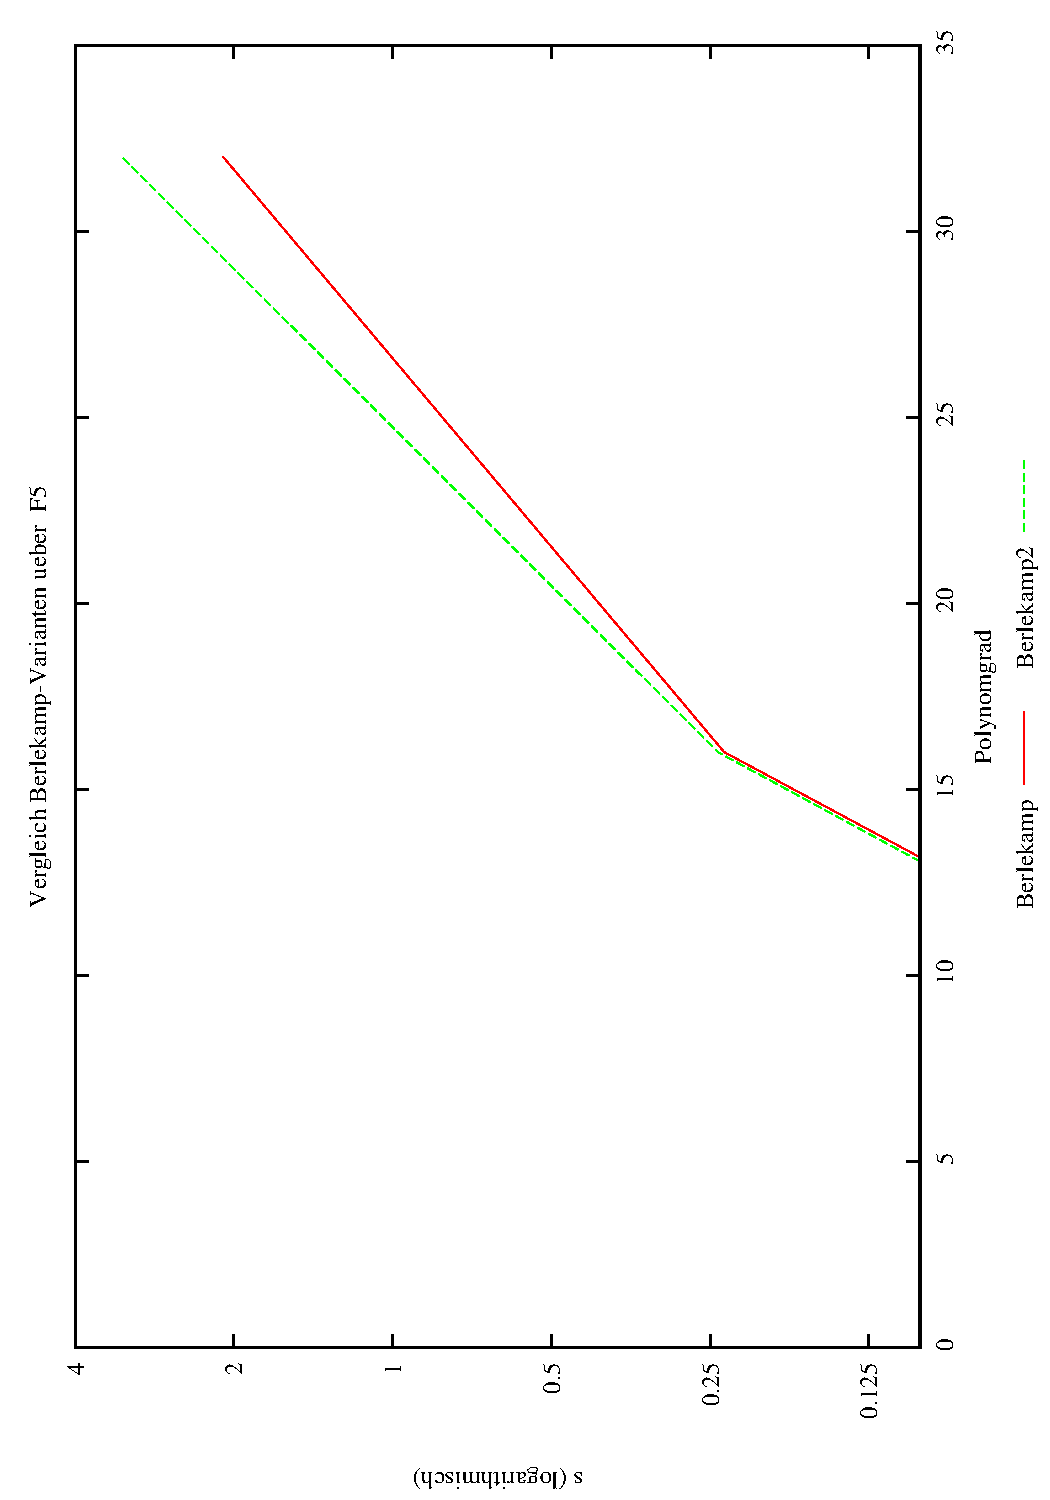
\includegraphics[width=0.7\textwidth,angle=-90]{plots/benchBerle_F5.pdf}
  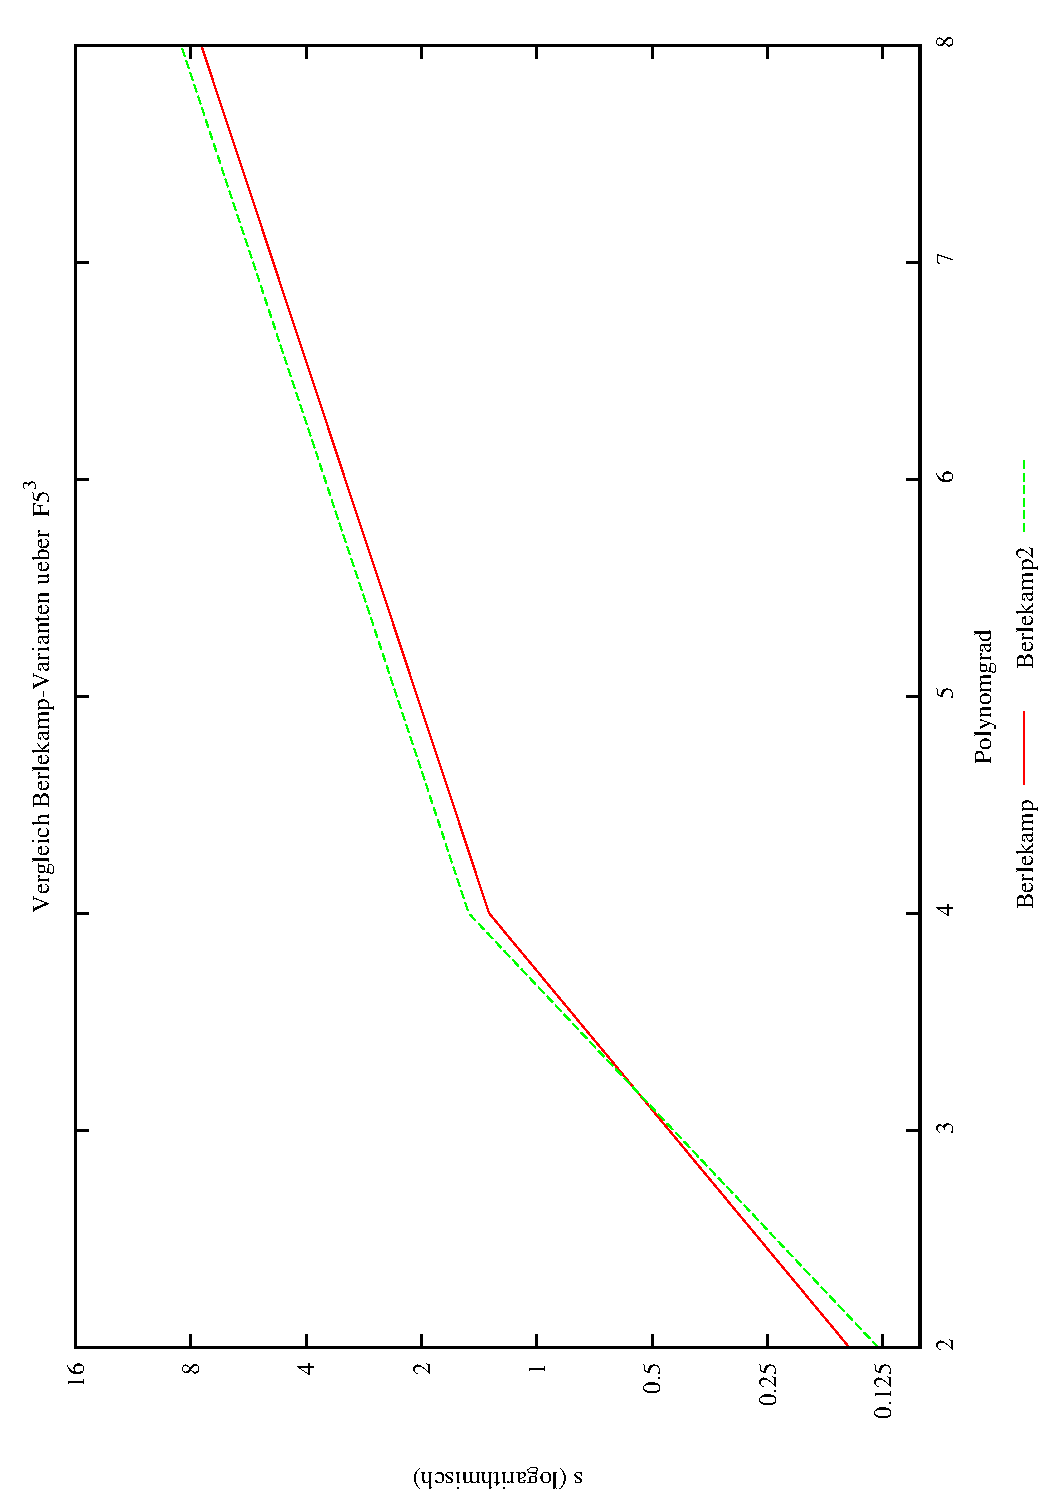
\includegraphics[width=0.7\textwidth,angle=-90]{plots/benchBerle_F53.pdf}
\end{figure}


\chapter{Performance}

%\chapter{Beispiel: 1}
%\input{../examples/Example.lhs}
%\chapter{Beispiel: Primitiv-normale-Elemente}
%\input{../examples/ExamplePrimitiveNormal.lhs}

%%%%%%%%%%%%%%%%%%%%%%%%%%%%%%%%%%%%%%%%%%%%%%%%%%%%%%%%%%%%%%%%%%%%%

%\addcontentsline{toc}{chapter}{Schluss}
%In den vorherigen Kapiteln konnten wir die Umsetzung einer Bibliothek von
Grundfunktionen auf endlichen Körpern in Haskell erläutern und demonstrieren.
Sicherlich sind die bisher implementierten Funktionen bei weitem nicht
ausreichend, um dieses Library als vollständig bezeichnen zu können. So ist
klar, dass die meisten Computer-Algebra-Systeme, was den Funktionsumfang
endlicher Körper betrifft, unserem kleinen Softwareprojekt überlegen
sind. Es gilt jedoch zu bemerken, dass wir gerade auf den Funktionsumfang für 
Polynome über endlichen Körpern, insbesondere was verschiedene
Multiplikations- und Faktorisierungsalgorithmen angeht, besonderes Augenmerk
gelegt haben.

\addsec{Wie könnte es weitergehen?}
Statt einer Schlussbemerkung drängt sich daher sicherlich die Frage nach einer
Fortsetzung des Projekts auf.

\paragraph{Erweiterung des Funktionsumfangs} Das Hinzufügen neuer
Funktionen könnte das Projekt fortsetzen. 
Bekanntlich existieren gerade für endliche Körper der Charakteristik 2 
spezielle Algorithmen, die weitaus effizienter sind, als ihre Pendents in
allgemeiner Charakteristik. Aus hauptsächlich
mathematisch interessierter Sicht ist dies vermutlich eine spannende
Aufgabe, da -- wie wir im Laufe des Projekts erkennen konnten -- die Syntax von
Haskell der Art und Weise mathematischer Notation besonders ähnlich ist.

\paragraph{Performance der Implementierung} Trotz der ,,Schönheit`` funktionaler
Programmierung mussten wir an vielen Stellen bemerken, dass das Konzept der
unveränderlichen Objekte auf Kosten der Performance geht. Insbesondere bei
großen Datenstrukturen, wie z.B. Polynomen über Körpererweiterungen (also
Polynome, deren Koeffizienten wiederum Polynome sind) oder auch Matrizen mit
polynomialen Einträgen, nimmt der \emph{garbage collector}, also dasjenige
Unterprogramm der Ausführung, das den Speicher nicht mehr benutzter Objekte
wieder frei gibt, einen großen, wenn nicht sogar den größten Teil der
Ausführungszeit ein. An diesem Punkt besteht sicherlich großes
Optimierungspotential. Ein Ansatz könnte es sein, an den berechnungsintensiven
Stellen von der Funktionalität abzuweichen und in \emph{Monaden}%
\footnote{Übrigens sind Monaden aus Sicht der Kategorientheorie sehr
interessante Objekte.}
(z.B. \autocite{haskellwiki:monaden}) zu wechseln. Alternativ könnte man
natürlich versuchen, \emph{mehr} statt weniger Funktionalität
zur Verbesserung der Laufzeit einzusetzen. Da, wie bereits öfters erwähnt,
Haskell Ausdrücke nicht auswertet, solange sie nicht de facto benötigt werden,
könnte man versuchen, die entstehenden \emph{Thunk}s 
(z.B. \autocite{haskellwiki:thunk}), also die noch nicht ausgewerteten Stellen,
zu vereinfachen. Beide Herangehensweisen sind sicherlich legitim, würden 
jedoch eine weitaus intensivere Einarbeitung in die tiefe Struktur von Haskell
erfordern und den Rahmen dieses Projekts sprengen. 

Obwohl an vielen Stellen sicherlich noch Optimierungspotential bezüglich der
Performance des Projekts besteht, möchten wir anmerken, dass Haskell im
Allgemeinen mindestens genauso schnell ist, wie andere Programmiersprachen.
(vgl. \autocite{haskellwiki:performance}) 

Nun möchten wir das Wort an 
Philip Greenspun und Autrijus Tang übergeben, um abschließend ein Gefühl für das
Programmieren in Haskell zu geben.

\begin{quote}
  \itshape SQL, Lisp, and Haskell are the only programming languages that 
  I've seen where one spends more time thinking than typing.
  \hfill\normalfont\sffamily\small Philip Greenspun%
  \footnote{%
  \url{http://blogs.law.harvard.edu/philg/2005/03/07/how-long-is-the-average-internet-discussion-forum-posting/}}
\end{quote}

\begin{quote}
  \itshape 
  Haskell is faster than C++, more concise than Perl, more regular than Python,
  more flexible than Ruby, more typeful than C\#, more robust than Java, and 
  has absolutely nothing in common with PHP.
  \hfill\normalfont\sffamily\small Audrey Tang%
  \footnote{\url{http://www.perl.com/pub/2005/09/08/autrijus-tang.html?page=2}}
\end{quote}


%%%%%%%%%%%%%%%%%%%%%%%%%%%%%%%%%%%%%%%%%%%%%%%%%%%%%%%%%%%%%%%%%%%%%
\pagebreak
\printbibliography

\appendix
\addcontentsline{toc}{chapter}{Anhang}


\newpage\thispagestyle{empty}
\begin{center}
\includegraphics[width=0.9\textwidth]{qrcode.eps}
https://github.com/maximilianhuber/softwareProjekt/
\end{center}
% vim:set ft=tex foldmethod=marker foldmarker={{{,}}}:


\end{document}
% vim:set ft=tex foldmethod=marker foldmarker={{{,}}}:
